\documentclass[english,11pt]{beamer}

\def \draft {1}




\DeclareMathOperator{\Cov}{Cov}
\DeclareMathOperator{\Var}{Var}
\DeclareMathOperator{\E}{\mathbb{E}}
\DeclareMathOperator{\Proba}{\mathbb{P}}

\newcommand{\Covb}[2]{\ensuremath{\Cov\!\left[#1,#2\right]}}
\newcommand{\Eb}[1]{\ensuremath{\E\!\left[#1\right]}}
\newcommand{\Pb}[1]{\ensuremath{\Proba\!\left[#1\right]}}
\newcommand{\Varb}[1]{\ensuremath{\Var\!\left[#1\right]}}

% norm
\newcommand{\norm}[1]{\| #1 \|}

\newcommand{\indep}{\rotatebox[origin=c]{90}{$\models$}}




\usepackage{mathptmx,amsmath,amssymb,graphicx,bibentry,bbm,babel,ragged2e}

\makeatletter

\usepackage{ifthen}

\newcommand{\noun}[1]{\textsc{#1}}
\newcommand{\jitem}[1]{\item \begin{justify} #1 \end{justify} \vfill{}}
\newcommand{\sframe}[2]{\frame{\frametitle{#1} #2}
\ifthenelse{\draft=1}{\frame{}}{}
}

\newenvironment{centercolumns}{\begin{columns}[c]}{\end{columns}}
%\newenvironment{jitem}{\begin{justify}\begin{itemize}}{\end{itemize}\end{justify}}


% -> in sframe
%\newcommand{\eframe}{
%    \ifthenelse{\draft=1}{\sframe{}{}}{}
%}




\usetheme{Warsaw}
\setbeamertemplate{footline}[text line]{}
\setbeamercolor{structure}{fg=purple!50!blue, bg=purple!50!blue}

\setbeamersize{text margin left=15pt,text margin right=15pt}

\setbeamercovered{transparent}


\@ifundefined{showcaptionsetup}{}{%
 \PassOptionsToPackage{caption=false}{subfig}}
\usepackage{subfig}

\usepackage[utf8]{inputenc}
\usepackage[T1]{fontenc}



\makeatother

\begin{document}


\title{Identification de causalités dans des données spatio-temporelles}

\author{J.~Raimbault$^{1,2}$\\
\texttt{juste.raimbault@parisgeo.cnrs.fr}
}


\institute{$^{1}$UMR CNRS 8504 G{\'e}ographie-cit{\'e}s\\
$^{2}$UMR-T IFSTTAR 9403 LVMT
}


\date{Séminaire LAET\\\smallskip
9 janvier 2018
}

\frame{\maketitle}





%%%%%%%%%%%%%%%%%%%
%% ABSTRACT

%\textbf{Mots-clés : }\textit{Causalité Spatio-temporelle ; Interactions Réseaux-Territoires ; Morphogenèse Urbaine ; Grand Paris ; Afrique du Sud ; Réseaux Ferré Français ; Co-évolution}

%Cette présentation contribue à la compréhension des processus spatio-temporels fortement couplés, en proposant une méthode générique basée sur la causalité de Granger. Plus précisément, la fouille de donnée et l'analyse spatiale sont utilisées pour revisiter l'étude des motifs de corrélations retardées, ce qui permet ainsi de comprendre les relations causales faibles entre différentes composantes des systèmes territoriaux.

%La méthode est validée dans un premier temps sur des données synthétiques, par l'identification de régimes de causalité et de leur diagramme de phase pour un modèle de morphogenèse urbaine couplant croissance du réseau et de la densité. Les graphes de relations causales entre variables qui sont obtenus ne sont pas reliés de manière simple aux paramètres régissant les interactions microscopiques, ce qui témoigne de la capture d'une causalité complexe par la méthode.

%L'application au cas des projets de transport du Grand Paris suggère différents liens entre les dynamiques territoriales, plus particulièrement socio-économiques et foncières, et la croissance anticipée du réseau, comme par exemple un processus de spéculation immobilière dans les quartiers des gares planifiées. Nous illustrons d'autres applications sur des temporalités plus longues : dans le cas des dynamiques d'accessibilité ferroviaire et de population urbaine en Afrique du Sud de 1911 à 1990, nous démontrons une inversion du sens de la causalité coïncidant avec la mise en place des politiques d'apartheid, suggérant un effet de celles-ci au second ordre, c'est à dire sur les relations dynamiques entre réseaux et territoires. D'autre part, l'application à la France entre 1830 et 1999 avec le réseau ferroviaire ne fournit quant à elle aucune corrélation significative, confirmant qu'il n'est dans certains cas pas possible d'établir des relations claires.

%Nous discutons finalement ces résultats en les plaçant dans la perspective plus large de la co-évolution des réseaux de transport et des territoires, dont nous donnons une définition ainsi que des pistes de modélisation. L'ensemble de ce travail propose ainsi un regard original sur la question des effets structurants des infrastructures de transport.



%%%%%%%%%%%%%%%%%
\section{Introduction}
%%%%%%%%%%%%%%%%%




\sframe{Interactions entre réseaux et territoires}{

% The study of strongly coupled spatio-temporal processes implies to understand tangled intrications generally highly difficult to isolate. These interactions are the essence of complexity approaches, and are indeed at the origin of the emergent behavior of the system. They make sense as an object of study in itself and a separation of processes appears then contradictory with an integrated view of the system. In the case of territorial systems, the example of interactions between transportation networks and territories is a perfect allegory of this phenomenon: methods developed in the seventies aimed at isolating the ``structuring effects'' of a transportation infrastructure~\cite{bonnafous1974methodologies} have later been unveiled as a political instrument and with a poor empirical support~\cite{offner1993effets}. The issue is still highly relevant today as it raises for example with the construction of new High Speed Rail lines in France~\cite{crozethalshs01094554}. The reality of territorial processus is in fact much more complicated than a simple causal relation between the introduction of a new infrastructure and spillovers on local development, but corresponds indeed to complex \emph{co-evolutive} processes~\cite{bretagnolletel00459720}. On long time scales and large spatial scales, some effects of dynamics reinforcement in system of cities by the insertion within networks have been shown by the application of the Evolutive Urban Theory~\cite{espacegeo2014effets}, showing that the disentangling is sometimes possible through a more global understanding of the system. At an other scale, still for relations between networks and territories, we can point at the relations between mobility practices, urban sprawl et ressource localisation in a metropolitan framework~\cite{cerqueira2017inegalites} that are as much complex. This kind of issue is naturally present in other fields: in Economic Geography, the example of links between innovation, local spillovers of knowledge and aggregation of economic agents is a typical illustration of spatio-temporal economic processes exhibiting circular causalities difficult to disentangle~\cite{audretsch1996r}. Specific methods are introduced, as the use of statistical instruments: \cite{aghion2015innovation} shows that the geographical origin of US Congress members that attribute local subsidies is a powerful instrumental variable to link innovation and income inequalities for higher incomes, what confirms that the significant correlation between the two is indeed a causality of innovation on inequalities.

\centering


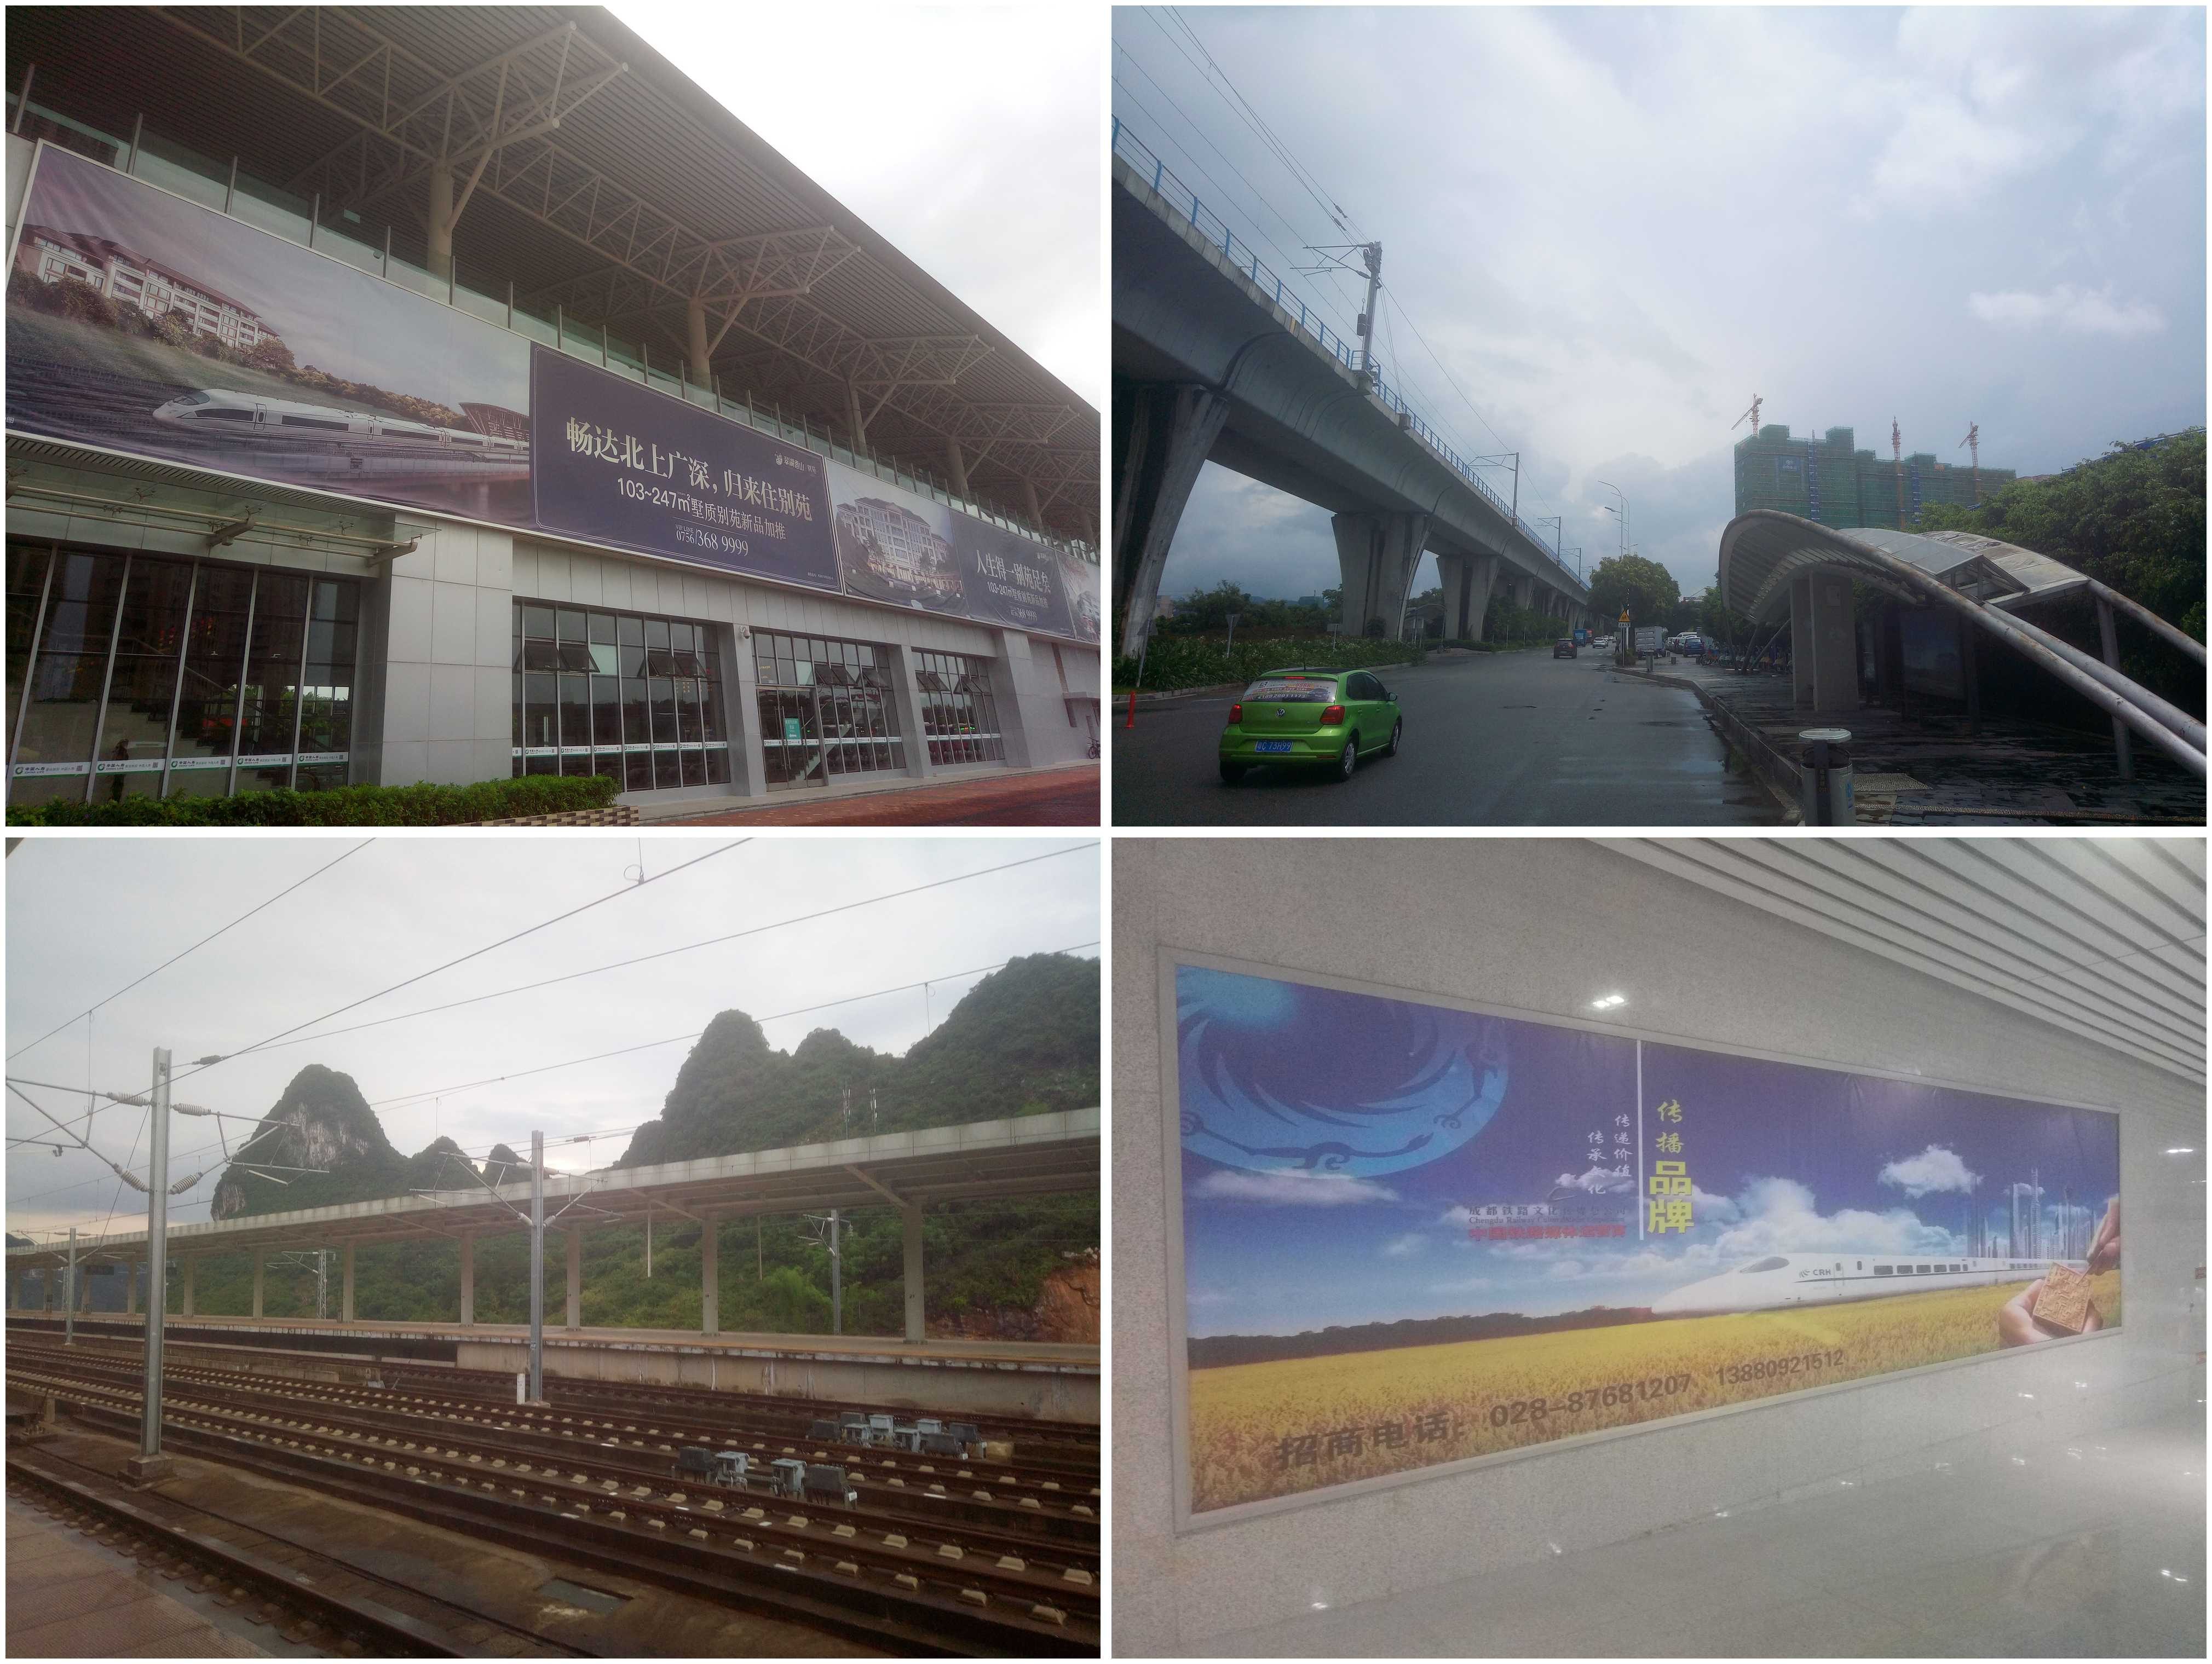
\includegraphics[width=0.43\textwidth]{figures/1-3-1-fig-qualitative-hsr}\hspace{0.1cm}
\includegraphics[width=0.55\textwidth]{figures/tod}

\bigskip

\textit{Un travail de terrain dans le Delta de la Rivière des Perles montre des manifestations locales des interactions entre réseaux de transport et territoires}

}

\sframe{Effet structurants des infrastructures}{


\justify

\textit{De \cite{bonnafous1974methodologies} à \cite{offner1993effets} : quels effets de structure des infrastructures de transport sur les territoires ?}

\bigskip
\bigskip

$\rightarrow$ Existence de processus co-évolutifs \cite{bretagnolletel00459720}

\medskip

$\rightarrow$ A petite échelle et sur le temps long, existence de dynamiques structurelles des systèmes urbains \cite{espacegeo2014effets}

\medskip

$\rightarrow$ La question des causalités circulaires revient à toutes les échelles (e.g. échelle métropolitaine et mobilité \cite{cerqueira2017inegalites}) et dans différents domaines (retombées locales et innovation \cite{audretsch1996r})



}


\sframe{Causalité en Géographie}{

\justify

% Strong coupling in space and time generally implies a notion of causality, that geography has always studied: \cite{loi1985etude} shows that fundamental issues tackled by contemporary theoretical geography (isolation of objects, link between space and causal structures, etc.) were already implicit in Vidal's classical geography. Beside, \cite{claval1985causalite} criticizes the new determinisms having emerged, in particular the one advocated by some scholars of systemic analysis: in its beginning, this approach inherited from cybernetics and thus of a reductionist vision implying a determinism even for a probabilistic formulation. Claval observes that works contemporary to his writings could allow to capture the complexity that characterizes human decisions: the Prigogine School and the Theory of Catastrophes by René Thom. This viewpoint is extremely visionary, since as Pumain recalls in~\cite{pumain2003approche}, the shift from system analysis to self-organisation and complexity has been long and progressive, and these works have played a fundamental role for it. François Durand-Dastès sums up this picture more recently in~\cite{durand2003geographes}, by focusing on the importance of bifurcations and path-dependency in the initial moments of the constitution of a system that he defines as \emph{systemogenesis}. This type of complex dynamics generally implies a co-evolution of system components, that can be understood as circular causalities between processes: the issue of identifying them is thus crucial regarding the notion of causality for contemporary complex geography.


$\rightarrow$ La Géographie classique s'intéressait déjà à des liens causaux dans l'espace \cite{loi1985etude}

\bigskip

$\rightarrow$ \cite{claval1985causalite} : au delà de la causalité réductionniste en analyse systémique

\bigskip

$\rightarrow$ La systèmogenèse introduite par \cite{durand2003geographes} se concentre sur la dynamique et les dépendances au chemin

\bigskip

$\rightarrow$ Vers une approche complexe de la causalité ? \cite{morin1976methode}

% -> reserve slide on morphogenesis.


}

\sframe{Approches empiriques existantes}{

\justify

%In the particular case of relations between network and territories, studies mainly in econometrics have tried to establish causality relationships between variables linked to these two objects. For example, \cite{levinson2008density} explains for the case of London population and connectivity to network variables by these same variables lagged in time, unveiling circular causal effects. \cite{doi10.1068/b39089} uses similar techniques for a region in Italy with historical data on long time, but stays moderate on possible conclusions of systematic effects by recalling the importance of historical events on the estimated relations. \cite{cuthbert2005empirical} proceeds to econometric estimations of reciprocal influence, and concludes that in their Canadian case study at a sub-regional scale, the development of the network induces the development of land-use but not the contrary. Space and time scales influence thus significantly the results of such analysis. \cite{koninghal-00962384} proposes an estimation of relations between the existence of a High Speed Rail connection and economic variables on French Urban Units, and shows a negative effect of the connection itself, after controlling on the endogenous nature of the connection by a selection model, and a significant effect of the characteristics of Urban Units. This work stays limited as it takes neither a time lag larger than one time step nor spatial relations between entities. Finally, still in the same spirit but without explicit inclusion of space, \cite{MANCMANC1073} shows on long time a causality link between infrastructure stock and economic growth on a global panel, but that these effects are moderated locally by under or over-investments.

\textbf{Réseaux de transports et territoires}

\begin{itemize}
	\item\justify Corrélations retardées : \cite{levinson2008density} Population et connectivité au réseau à Londres ; \cite{doi10.1068/b39089} données historiques en Italie du Nord
\end{itemize}
\begin{itemize}
	\item\justify Variables instrumentales : \cite{duranton2012urban} Réseau routier et emplois aux Etats-Unis ; \cite{berger2017locomotives} effet significatif du réseau ferré suédois sur les trajectoires urbaines
\end{itemize}



% The regimes under which identification of causalities are relevant are not obviously known. These will depend of the definitions used, as well as available methods for which we give now a few examples. \cite{liu2011discovering} proposes to detect spatio-temporal relations between perturbations of trafic flows, introducing a particular definition of causality based on correspondance of extreme points. Associated algorithms are however specific and difficult to apply to other kind of systems. The use of spatio-temporal correlations has been shown to have in some cases a strong predictive power for trafic flows~\cite{min2011real}. Also in the field of transportation and land-use, \cite{xie2009streetcars} applies a Granger causality analysis, that can be interpreted as lagged correlation, to show for a case study that network growth inducts urban development and is itself driven by externalities such as mobility habits. Neuroscience has developed numerous methods answering similar issues. \cite{luo2013spatio} defines a generalized Granger causality that takes into account non-stationarity and applies to abstracts regions produced by functional imaging. This kind of method is also developed in Computer Vision, as illustrated by \cite{ke2007spatio} that exploits spatio-temporal correlations of forms and flows between successive images to classify and recognize actions. Applications can be quite concrete such as compression of video files by extrapolation of motion vectors~\cite{chalidabhongse1997fast}. In all these cases, the study of spatio-temporal correlations meets the weak notions of causality described above.

\medskip

\textbf{Corrélations spatio-temporelles}

\begin{itemize}
	\item Méthode de correspondance pour les flux de trafic \cite{liu2011discovering}
	\item Causalité de Granger généralisée en neurosciences \cite{ke2007spatio}
	\item Corrélations spatio-temporelles en Vision par Ordinateur \cite{ke2007spatio}
\end{itemize}



}

\sframe{Contexte}{

% insist on datamining approach - because Granger causality seen and reseen : structure of data/unsupervised

%  This contribution aims to explore the possibility of a similar methods for spatio-temporal data exhibiting a priori complex circular causalities, and thus to realize the difficult exercise to couple a certain level of simplicity with a grasping of complexity. We introduce therefore a method to analyse spatio-temporal correlations, similar to a Granger causality estimated in space and time. The robustness of the method is demonstrated in a systematic way by the application to a complex model of simulation of urban morphogenesis, what leads to the unveiling of distinct causality regimes in the phase space of the model. We also include the application to an empirical case study, what positions this work at the interface between knowledge domains of methodology, modeling and empirical within the epistemological framework introduced by~\cite{2017arXiv170609244R}.

$\rightarrow$ Généricité et opérationnalité des approches existantes ?

\medskip

$\rightarrow$ Capturer la complexité simplement ?

\medskip

$\rightarrow$ A l'interface des domaines de connaissance (méthodologie, modélisation et empirique) \cite{2017arXiv170609244R}


\bigskip
\bigskip

\textbf{Objectif de recherche : } 

\textit{Exploration d'une méthode générique basée sur les motifs des corrélations spatio-temporelles retardées : notion de causalité de Granger ; validation sur données synthétiques.}


% The rest of this paper is organized as follows: the generic framework of the method is described in the next section. We then apply it to a synthetic dataset to partially validate it and test its potentialities, what allows us to apply it then to the real case study of Grand Paris transportation network. We finally discuss to proximity with existing methods and possible developments.



}





%%%%%%%%%%%%%%%%%
\section{Méthodes et Résultats}
%%%%%%%%%%%%%%%%%


\sframe{Aperçu de la méthode}{

\centering

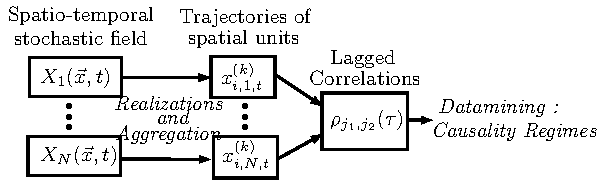
\includegraphics[width=\linewidth]{figures/causality_regimes}

}


\sframe{Formalisation de la méthode}{

Estimateur de corrélation $\hat{\rho}$ s'appliquant dans le temps, l'espace, et les répétitions, i.e. la covariance est estimée par $\hat{\Cov}\left[X,Y\right] = \hat{\mathbb{E}}_{i,t,k}\left[XY\right] - \hat{\mathbb{E}}_{i,t,k}\left[X\right]\hat{\mathbb{E}}_{i,t,k}\left[Y\right]$

\bigskip

Corrélations retardées définies comme

\begin{equation}
\rho_{\tau}\left[X_{j_1},X_{j_2}\right] = \hat{\rho}\left[x^{(k)}_{i,j_1,t - \tau},x^{(k)}_{i,j_2,t}\right]
\end{equation}

\bigskip

%We formalize here the method in a generic way, based in a weak formulation of Granger causality, to try to identify causal relations in spatial systems. Let $X_j(\vec{x},t)$ spatio-temporal unidimensional random processes, which realizations occur in space and time. We give a set of fundamental spatial units  $(u_i)$ that can be for example raster cells or any paving of the geographical space. We assume the existence of functions $\Phi_{i,j}$ allowing to make the correspondance between the realization of each components and spatial units, possibly through a first spatial aggregation or by a more elaborated process driven by a network for example. A realization of a system is given by a set of trajectories for each process $x_{i,j,t}$, and we write a set of realizations $x^{(k)}_{i,j,t}$ (accessible by stochastic repetitions in the case of a model of simulation for example, or by assumption of comparability of territorial sub-systems in real cases). We assume to have a correlation estimator $\hat{\rho}$ applying in time, space and repetitions, i.e. $\hat{\rho}\left[X,Y\right] = \hat{\mathbb{E}}_{i,t,k}\left[XY\right] - \hat{\mathbb{E}}_{i,t,k}\left[X\right]\hat{\mathbb{E}}_{i,t,k}\left[Y\right]$. It is important to note here the hypothesis of spatial and temporal stationarity, that can however easily be relaxed in the case of local stationarity. Furthermore, spatial auto-correlation is not explicitly included, but is taken into account either by the initial spatial aggregation is the characteristic scale of units is larger than the one of neighborhood effects, either by an adequate spatial estimator (weighted spatial statistics of type \emph{GWR}~\cite{brunsdon1998geographically} for example). It allows us to define the lagged correlation by 

%The lagged correlation is not symmetric, but we have directly $\rho_{\tau}\left[X_{j_1},X_{j_2}\right] = \rho_{-\tau}\left[X_{j_2},X_{j_1}\right]$. This measure is applied in a simple way: if $\textrm{argmax}_{\tau} \rho_{\tau}\left[X_{j_1},X_{j_2}\right]$ or $\textrm{argmin}_{\tau} \rho_{\tau}\left[X_{j_1},X_{j_2}\right]$ are ``clearly defined'' (both could be simultaneously), their sign will give the sense of causality between components $j_1$ and $j_2$ and their absolute value the propagation lag. The criteria for significance will depend on the case of application and of the estimator used, but can for example include the significance of the statistical test (Fisher test in the case of a Pearson estimator), the position of extremities of a confidence interval of a given level, or even an exogenous threshold $\theta$ on $\left|\rho_{\tau}\right|$ to ensure a certain level of correlation.

Le motifs de $\textrm{argmax}_{\tau} \rho_{\tau}\left[X_{j_1},X_{j_2}\right]$ ou de $\textrm{argmin}_{\tau} \rho_{\tau}\left[X_{j_1},X_{j_2}\right]$ (en les supposant clairement définis : e.g. significativité statistique, valeur seuil) capture le sens de la causalité entre $j_1$ et $j_2$

\medskip

$\rightarrow$ Datamining sur $\rho_\tau$ (possiblement paramétré comme $\rho_\tau^{(\omega)}$) pour explorer les motifs de causalité.

}


\sframe{Illustration pour 2 variables}{

\centering

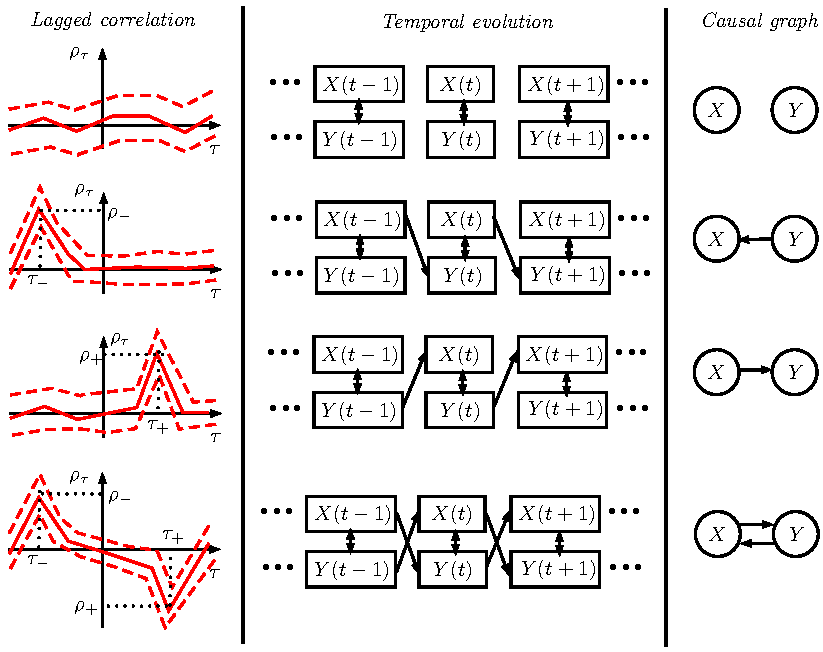
\includegraphics[height=0.9\textheight]{figures/causality_twovars.pdf}

}



\sframe{Validation basique}{

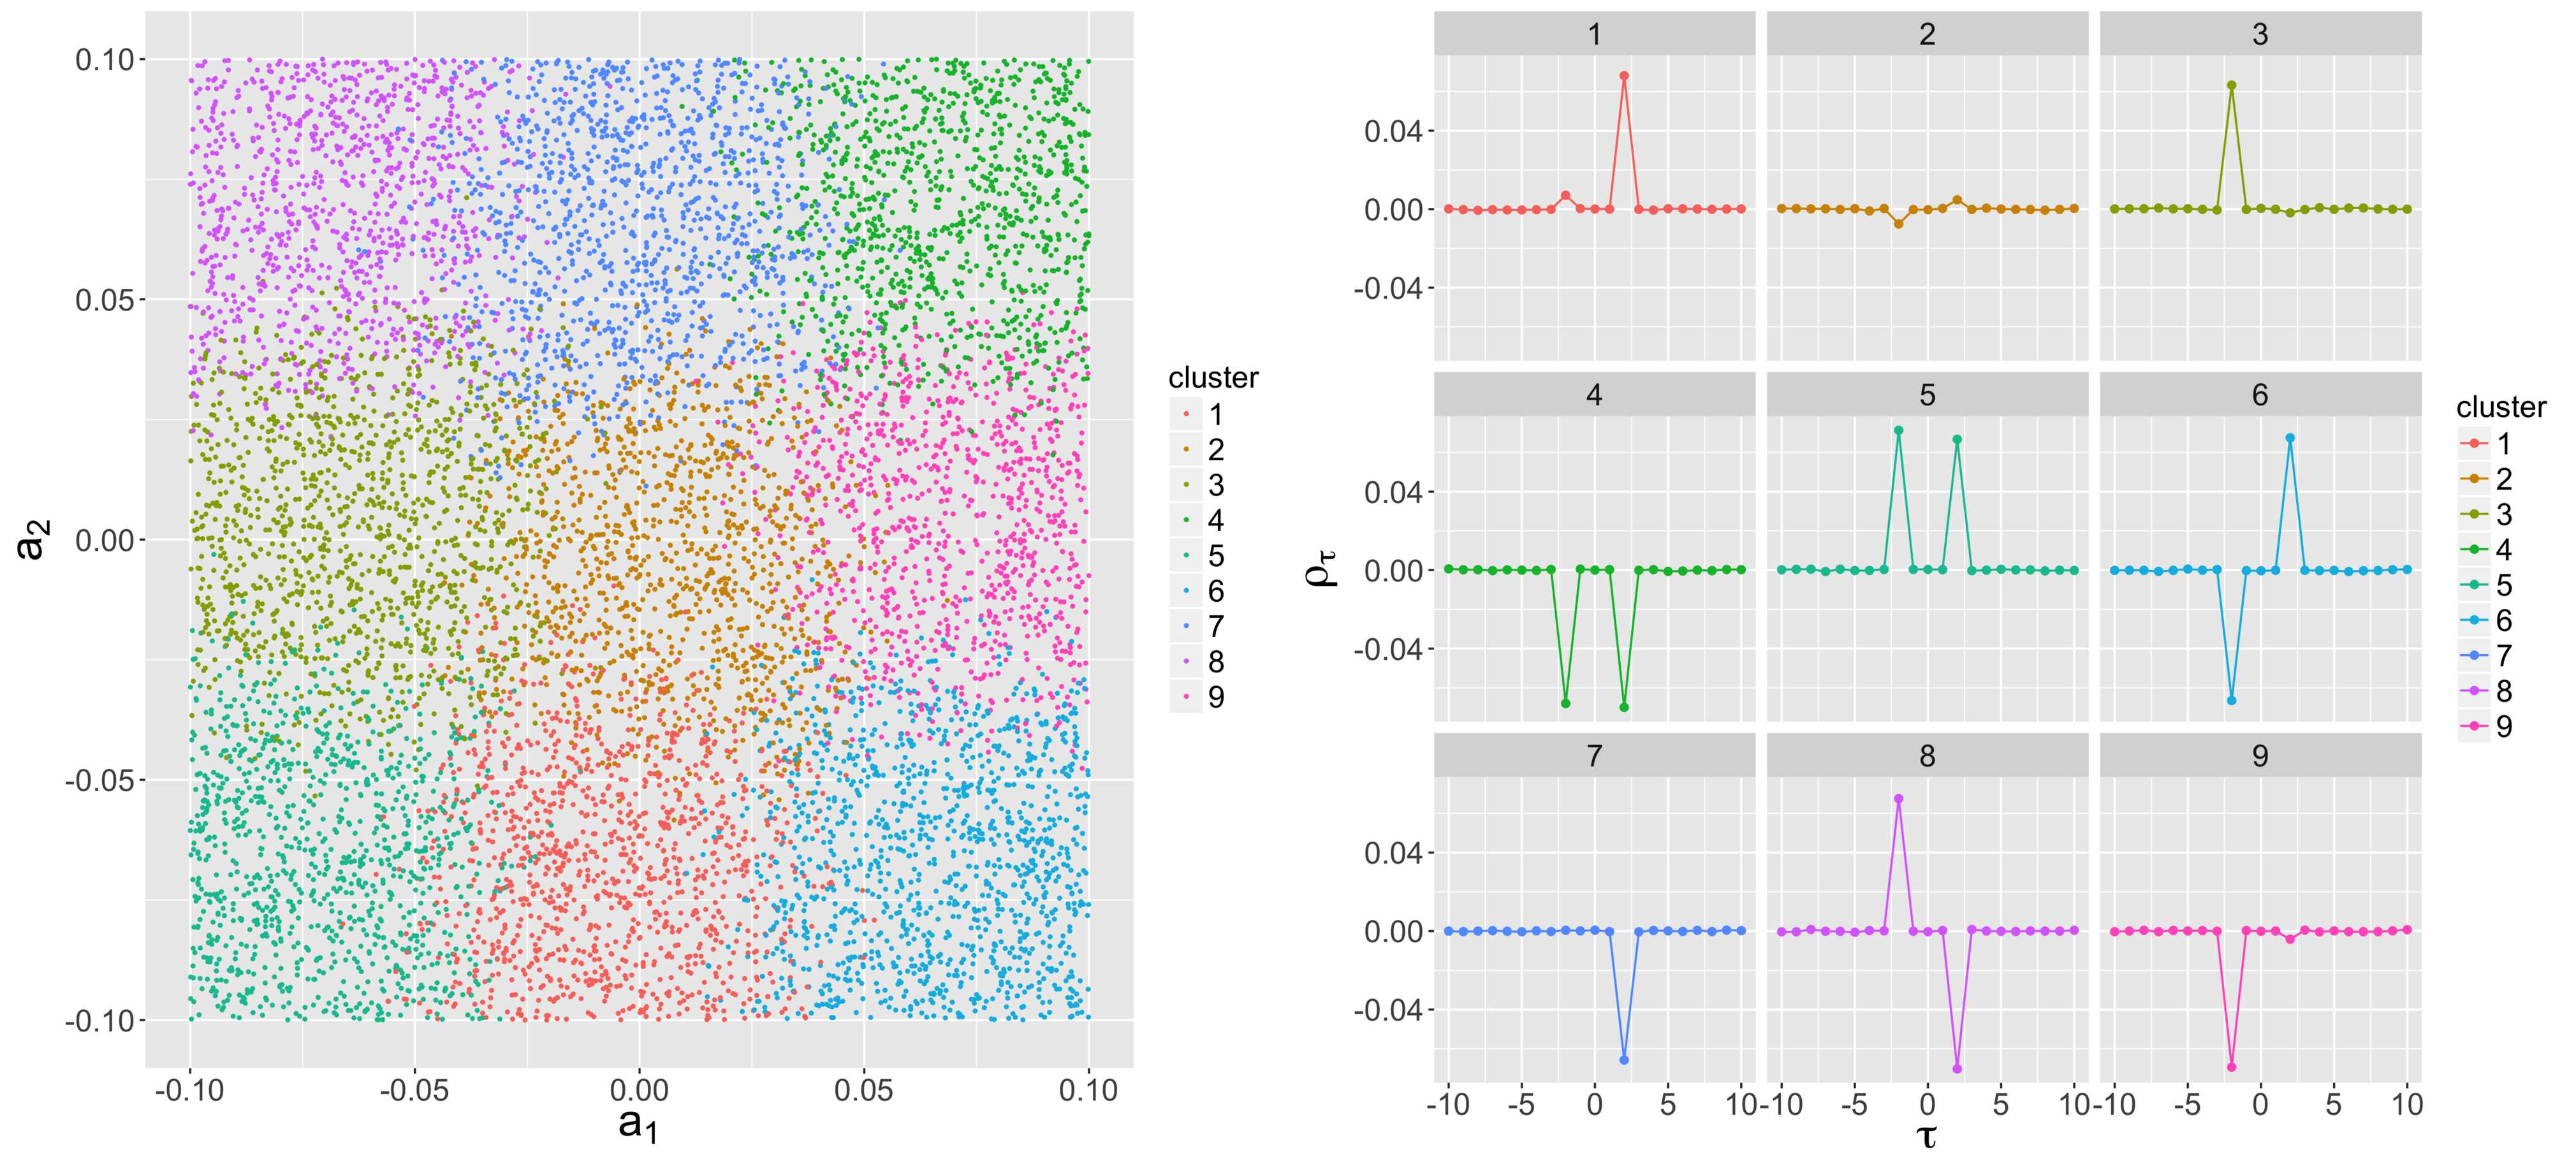
\includegraphics[width=\linewidth]{figures/4-2-2-fig-causalityregimes-arma.jpg}

\medskip

\textit{Données synthétiques : processus AR avec retard 2, termes croisés paramétrés par $(a_1,a_2) \in [-0.1,0.1]$ aléatoires.}

}




\sframe{Validation sur données synthétiques}{

% present strategy and rbd model

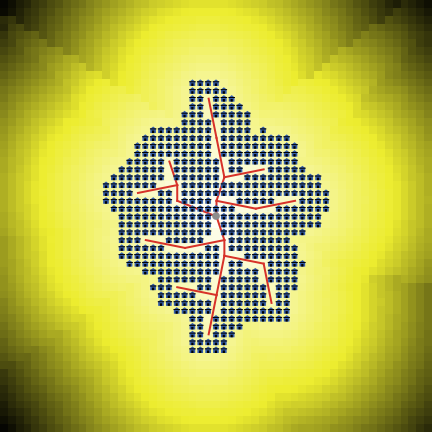
\includegraphics[width=0.32\textwidth]{figures/ex_60_wdens0_wroad1_wcenter1_seed272727}\hspace{0.1cm}
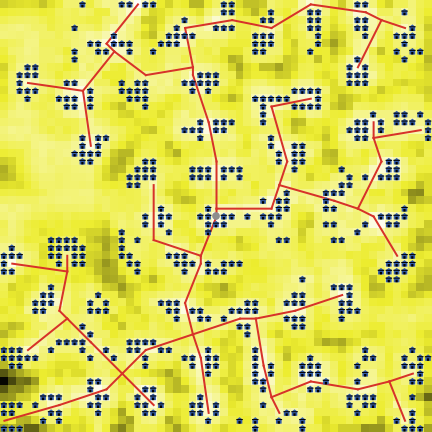
\includegraphics[width=0.32\textwidth]{figures/ex_60_wdens1_wroad1_wcenter0_seed272727}\hspace{0.1cm}
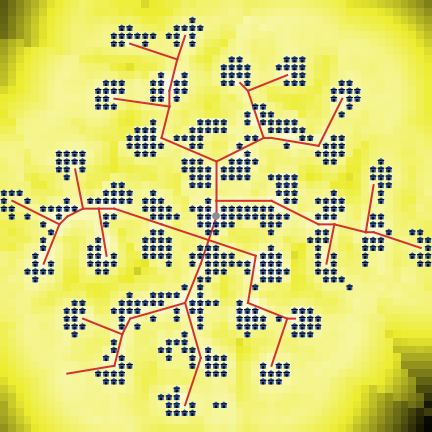
\includegraphics[width=0.32\textwidth]{figures/ex_60_wdens1_wroad1_wcenter1_seed272727}\hspace{0.1cm}

\medskip

\textit{Configurations urbaines synthétiques générées par un modèle de morphogenèse hybride issu de \cite{raimbault2014hybrid}}

}

\sframe{Description du modèle de morphogenèse}{

% plus de details sur le rbd
\begin{itemize}
\item Automate cellulaire: cellules d'une grille carrée $(L_{i,j})_{1\leq i,j\leq N}$
, occupées ou non (fonction \textrm{$\ensuremath{\delta(i,j,t)\in\{0,1\}}$)}
\end{itemize}
\vfill{}

\begin{itemize}
\item Réseau vectoriel $G(t)=(V(t),E(t))$ qui évolue,
incluant des centres urbains fixes $C_{0}\subset V(0)$ auxquels des activités
$a\in\{1,\ldots,a_{max}\}$ sont attribuées (propriétés fonctionnelles de l'environnement urbain).
\end{itemize}
\vfill{}

\begin{itemize}
\item Variables explicatives $(d_{k})_{1\leq k\leq K}$ définies sur les cellules, avec des poids associés $(\alpha_{k})_{1\leq k\leq K}$
(paramètres principaux du modèle), qui sont:

\begin{itemize}
\item $d_{1}$ densité autour de la cellule (dans un rayon fixé $r$)
\item $d_{2}$ distance à la route la plus proche
\item $d_{3}$ distance au centre le plus proche par le réseau
\item \textrm{$d_{4}(i,j,t)=\left(\frac{1}{a_{\max}}\sum_{a=1}^{a_{\max}}d_{3}(i,j,t;a)^{p_{4}}\right)^{1/p_{4}}$
}: accessibilité intégrée aux activités
\end{itemize}
\end{itemize}
\vfill{}


}

\sframe{Règles d'évolution}{

A chaque pas de temps :\vfill{}

\begin{itemize}
\item Etalement de la surface occupée : les meilleures $N$ cellules selon
la valeur du potentiel $v(i,j,t)=\frac{1}{\sum_{k}\alpha_{k}}\sum_{k=1}^{K}\alpha_{k}\;\frac{d_{k,\max}(t)-d_{k}(i,j,t)}{d_{k,\max}(t)-d_{k,\min}(t)}$
sont construites.\vfill{}

\item Adaptation du réseau : quand une nouvelle cellule est construite, si $d_{2}>\theta_{2}$, la cellule est connectée au réseau par une route directe.\vfill{}

\end{itemize}
}





\sframe{Profils de corrélations retardées}{

\includegraphics[width=\textwidth]{figures/regimes_1.png}

%\textit{Values of $\rho_{\tau}$ for all couples of three explicative variables (density, distance to center, distance to roads), for 8 extreme parameter points}

}


\sframe{Profils de corrélations retardées}{

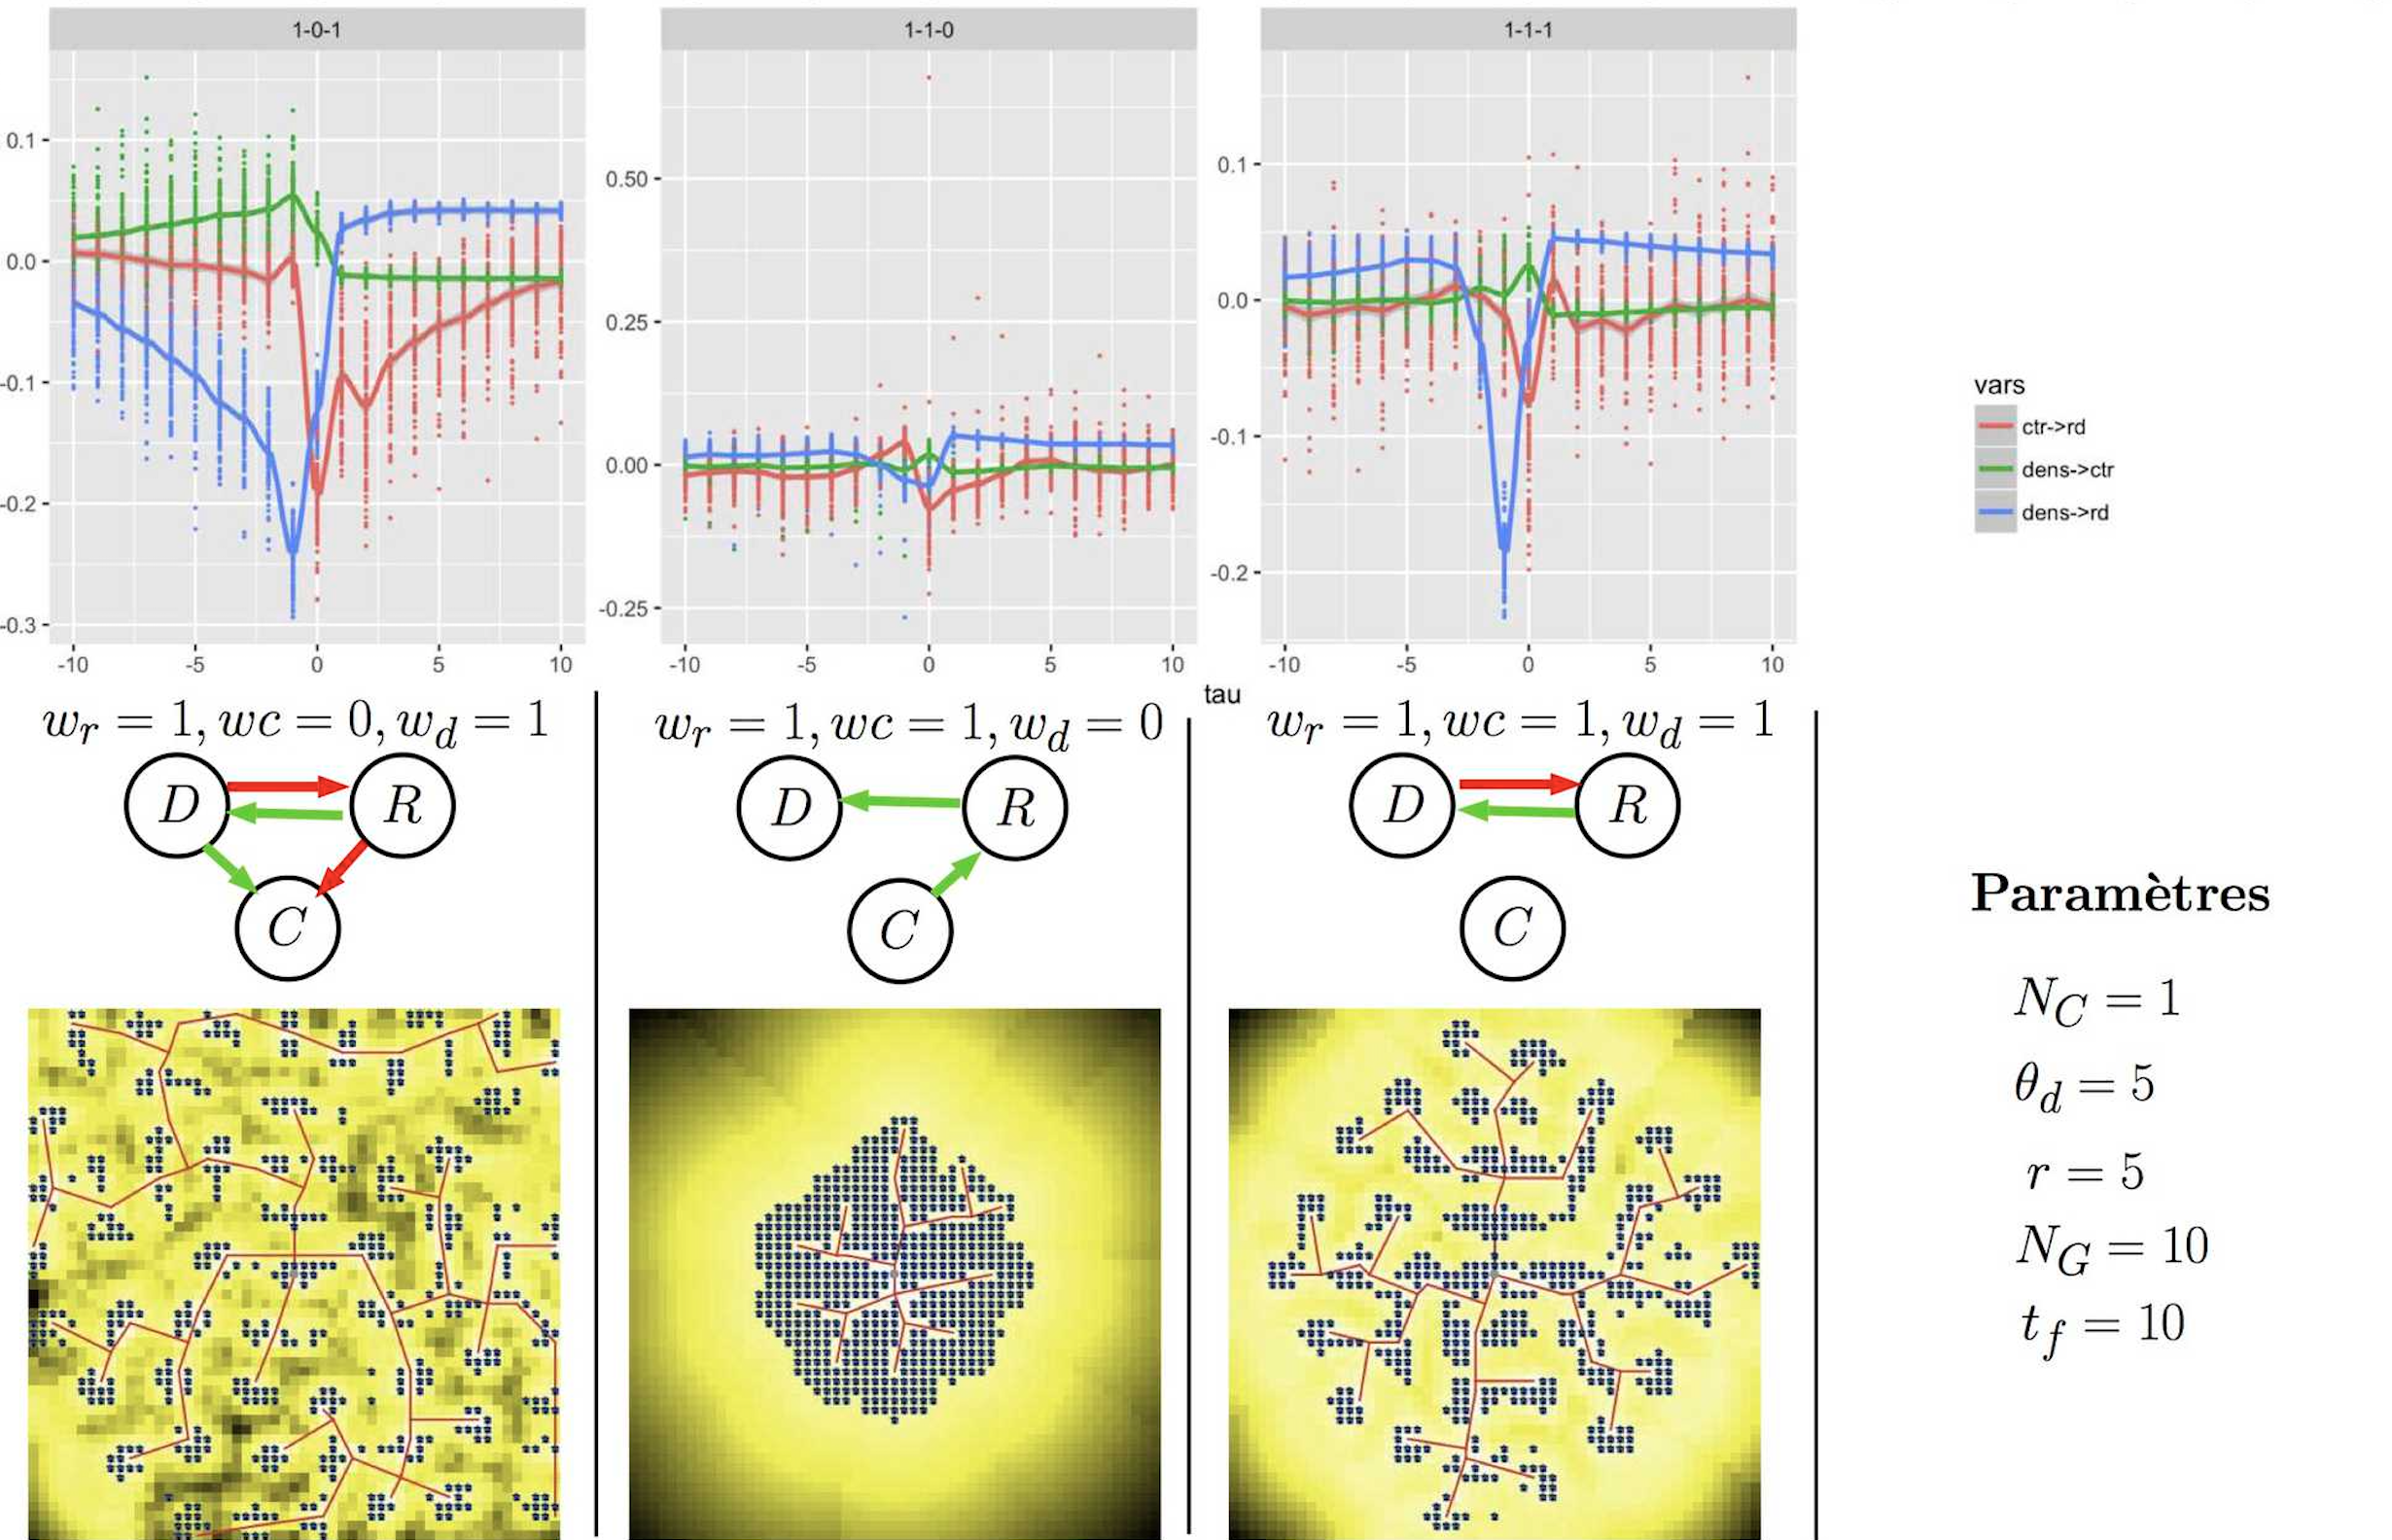
\includegraphics[width=\textwidth]{figures/regimes_2.png}

}


\sframe{Régimes endogènes de causalité}{

Exploration intensive de l'espace des paramètres du modèle (1000 points de paramètres x 100 répétitions) avec le logiciel OpenMole \cite{reuillon2013openmole}

\medskip

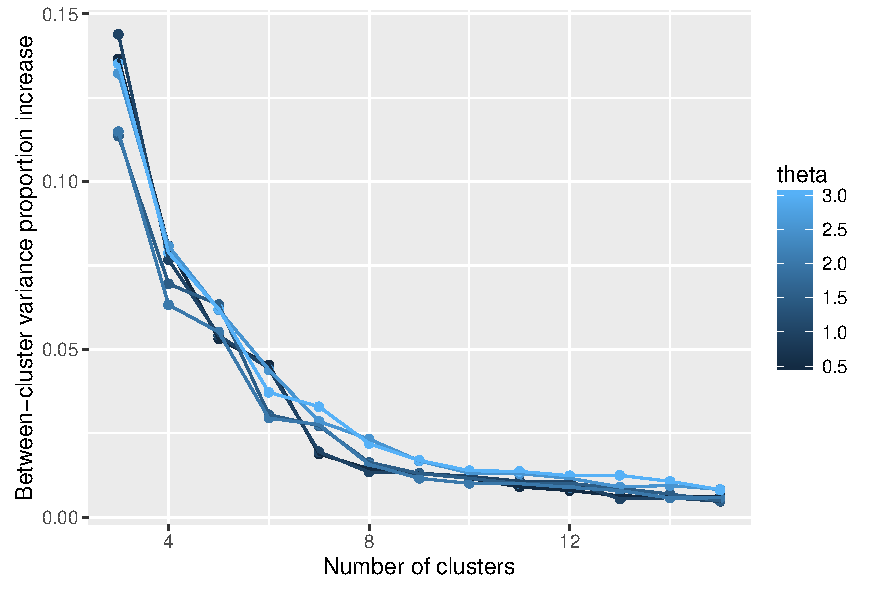
\includegraphics[width=0.52\textwidth]{figures/dccoef-knum_valuesFALSEtheta05-3}
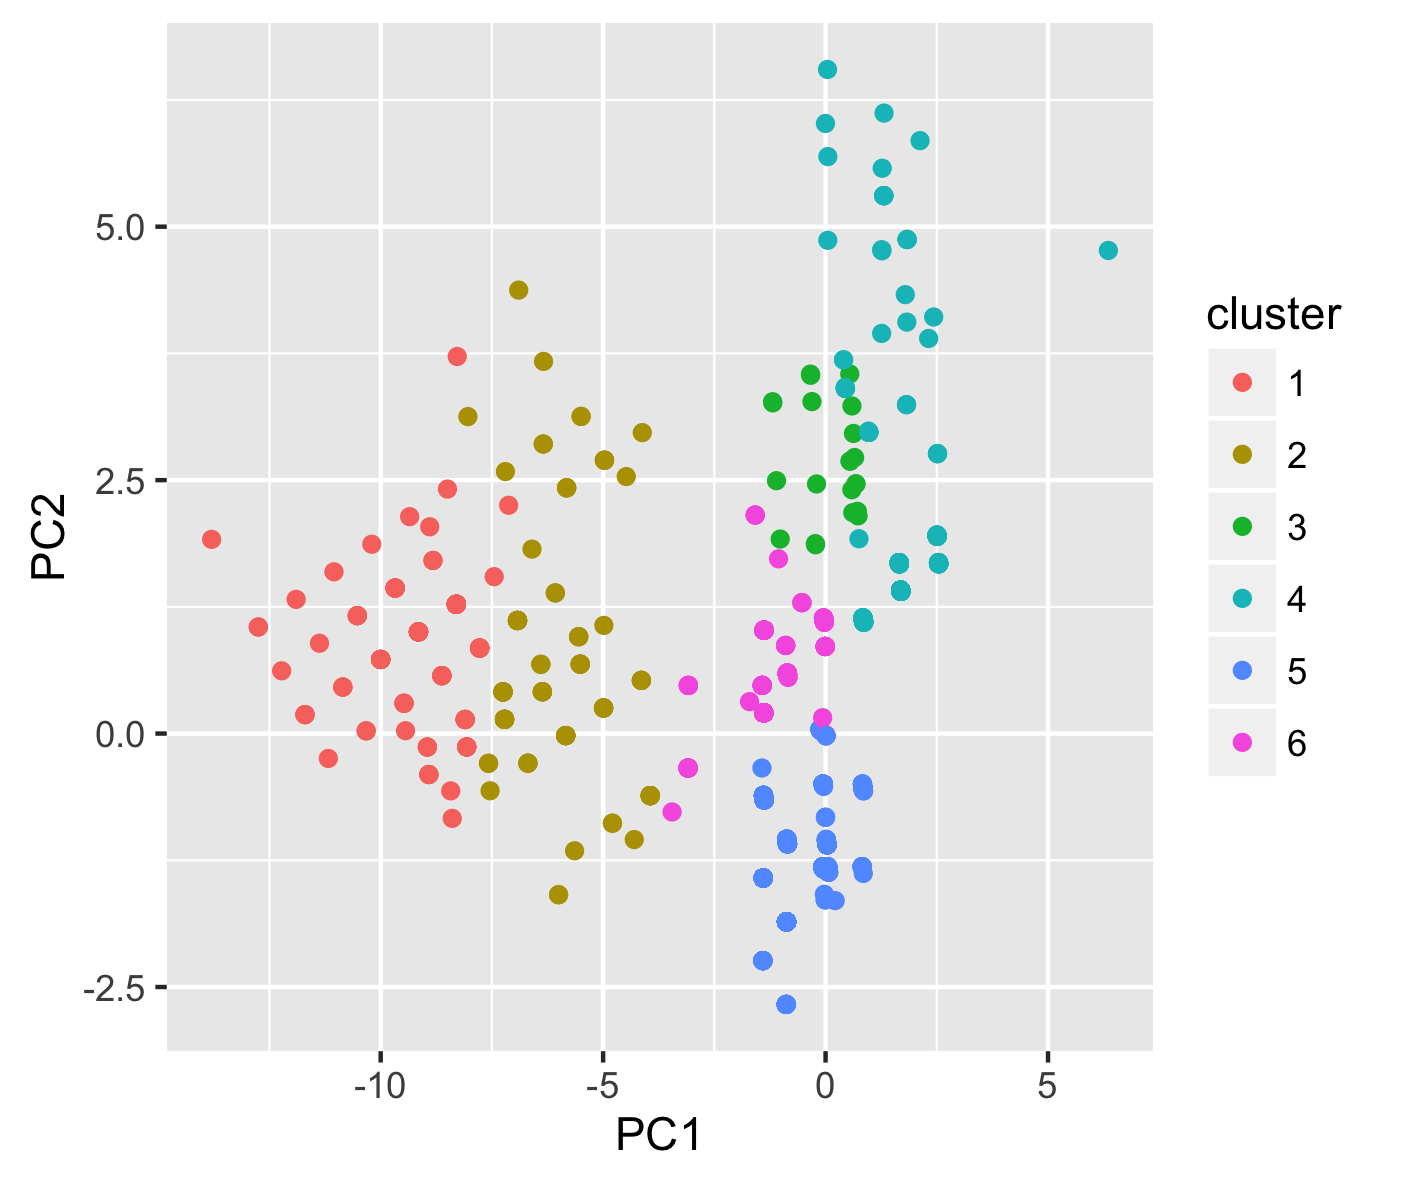
\includegraphics[width=0.44\textwidth]{figures/clusters-PCA-features_valuesFALSEtheta2_k6}

\footnotesize\textit{Classification non-supervisée (\textit{k-means} robustes) sur les caractéristiques $\tau_{min},\tau_{max}$ : (Gauche) Dérivée du coefficient de clustering en fonction du nombre de clusters $k$; (Droite) Visualisation en plan principal pour $k=6$.}

}

\sframe{Composition des régimes}{

\centering

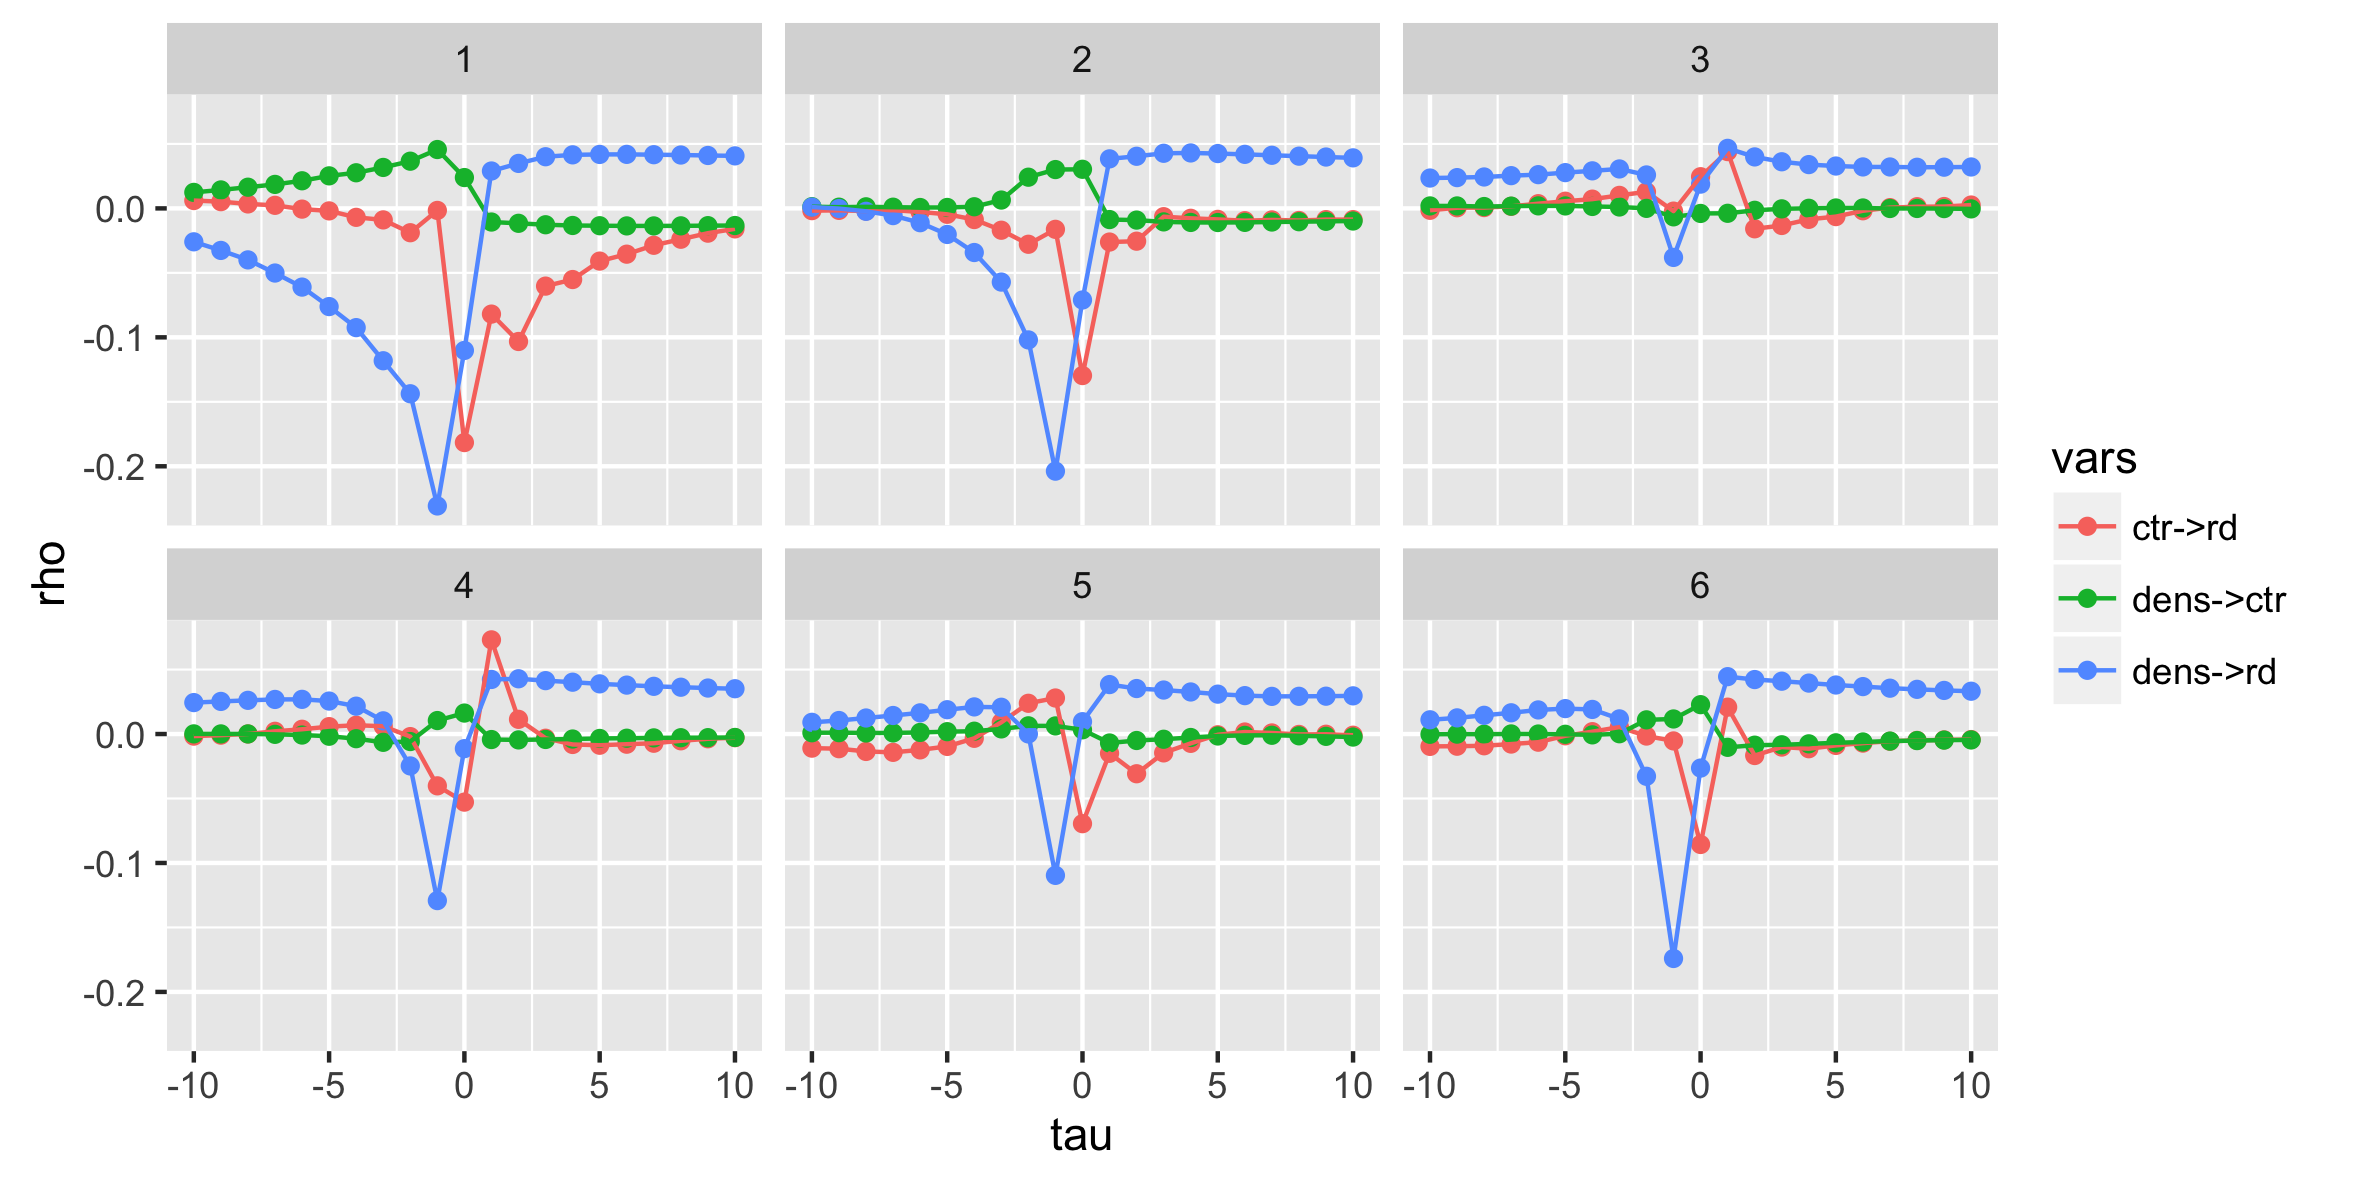
\includegraphics[width=\textwidth]{figures/clusters-centertrajs-facetclust_valuesFALSEtheta2_k6}

\textit{Valeurs des centres des clusters en termes de $\rho_{\tau}$}

}

\sframe{Interprétation des régimes}{

\centering

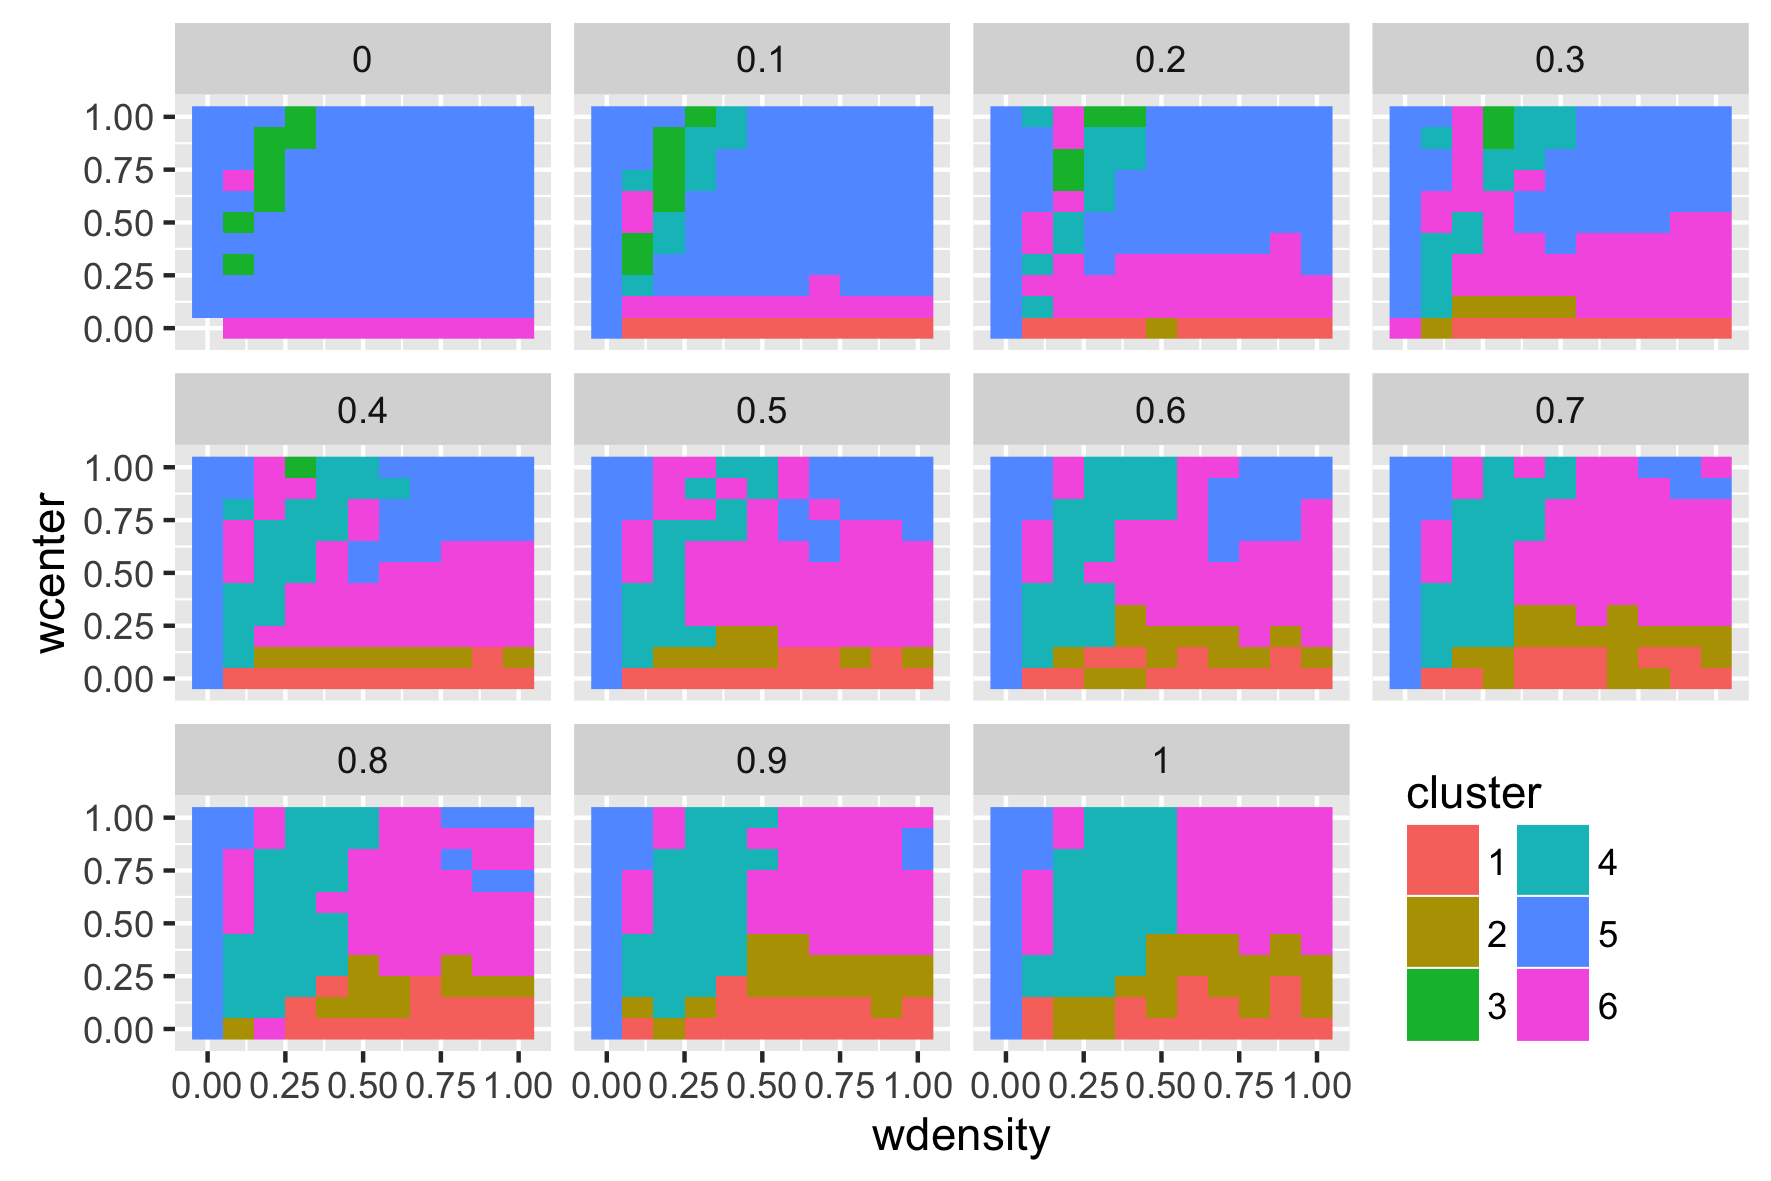
\includegraphics[width=0.9\textwidth]{figures/clusters-paramfacet_valuesFALSEtheta2_k6}

\textit{Position des clusters dans l'espace des paramètres $w_i$}


}


% This method must first be tested and partially validated, what we propose to do on synthetic data, what allows a more refined knowledge of the behavior of models~\cite{raimbaulthalshs01514415}. Echoing the example of relations between transportation networks and territories that introduced the research question before, we generate stylized urban configurations in which network and density mutually interact, and for which causalities are not obvious \emph{a priori} knowing the parameters of the generative model. \cite{raimbault2014hybrid} describes and explores a simple model of urban morphogenesis (the RBD model) that fits perfectly these constraints. Indeed, explicative variables of urban growth, processes of network extension and the coupling between urban density and the network are relatively simple. However, except for extreme cases (for example when distance to the center solely determines land value, the network will depend on density in a causal way; when only the distance to the network counts, the causality will be inverted), mixed regimes do not exhibit obvious causalities. It is for this reason an ideal case to test if the method is able to detect some. We use an applied implementation\footnote{available on the open repository of the project at \\\texttt{https://github.com/JusteRaimbault/CityNetwork/tree/master/Models/Simple/ModelCA}} of the original model, allowing to capture the values of studied variables for each cell of the cellular automaton and for each time step, and to calculate the lagged correlations in the sense described before, between variables of the model. We explore a grid of the parameter space of the RBD model, making the weight parameters for density, distance to center and distance toi network vary\footnote{The model works the following way: a value of cells is determined by the weighted average of these different explicative variables, value that determines the growth of new patches at the next time step.}, that we write respectively $(w_{d},w_{c},w_{r})$, in $\left[0;1\right]$ with a step of $0.1$. Other parameters are fixed to their default values given by~\cite{raimbault2014hybrid}. For each parameter value, we proceed to $N=100$ repetitions, what is enough for a good convergence of indicators. Explorations are done with the OpenMole software~\cite{reuillon2013openmole}, the large number of simulations (1,330,000) implying the use of a computation grid. We compute for all patches the lagged correlations with the unbiased Pearson estimator between the variations of the following variables\footnote{Computing the correlations directly on the variables makes no sense since their value has no absolute meaning.}: local density, distance to center and distance to network. The figure~\ref{fig:exrdb}  shows the behavior of $\rho_{\tau}$ for each couple of variable (undirected, $\tau$ taking negative and positive values), for the combination of extreme values of parameters. We can already see different regimes emerge: for example, $(1,0,1)$ leads to a causality of density on distance to center with a lag $\tau=1$, and a negative causality of density on distance to network with the same lag, whereas distance to the center and to the network are correlated in a synchronous manner. To study these behaviors in a systematic way, we propose to identify regimes endogenously, by using non-supervised classification. We apply a \emph{k-means} clustering, robust to stochasticity (5000 repetitions), with the following features: for each couple of variables, $\textrm{argmax}_{\tau} \rho_{\tau}$ and $\textrm{argmin}_{\tau} \rho_{\tau}$ if the corresponding value is such that $\frac{\rho_{\tau}-\bar{\rho}_{\tau}}{\left|\bar{\rho}_{\tau}\right|} > \theta$ with $\theta$ threshold parameter, 0 otherwise. The inclusion of supplementary features of values of $\rho_{\tau}$ does not significantly changes the results, these are therefore not taken into account to reduce the dimension. The choice of the number of clusters $k$ is generally a difficult problem in this kind of approach~\cite{hamerly2003learning}. In our case the system exhibit an convenient structure: the curves of inter-cluster variance proportion and its derivative in figure~\ref{fig:clustering}, as a function of $k$ for different values of $\theta$, show a transition for $\theta = 2$, what gives for the corresponding curve a break around $k=6$. A visual screening of clusters in a principal plan confirms the good quality of the classification for these values. A class corresponds then to a \emph{causality regime}, for which we can represent the phase diagram as a function of model parameters, and also cluster centers profiles (computed as the barycenter in the full initial space) in figure~\ref{fig:clustering}. The behavior obtained is interesting, as regions in the diagram corresponding to the different regimes are clearly delimited and connected. For example, we observe the emergence of regime 6 in which distance to network causes strongly the density in a negative way, but distance to the center causes distance to the network. Its maximal extent on $(w_d,w_r)$ is for an intermediate value $w_r=0.7$. Thus, to maximize the impact of network on density, the corresponding weight must not be maximized, what can be counter-intuitive at first sight. It illustrates the utility of the method in the case of circular causal relations difficult to entangle a priori. The regime 5, in which distance to network influences the density the same way, but the relation between distance to center and to the network is inverted, is also interesting, and predominates for low $w_r$ values. The regime 1 is an extreme one and corresponds to an isolated situation in which distance to the center has no role: this aspect dominates then totally the other interaction processes between density and network. This application on synthetic data demonstrate on one hand the robustness of the method given the consistence of obtained regimes, and realizes this way a much more finer qualification of model behavior than the one done in the original paper. In this precise case, it can be taken as an instrument of knowledge for relations between networks and territories in itself, allowing the test of assumption or the comparison of processes in the stylized model.





\sframe{Application: Cas d'étude}{

% We propose an application on a real case study, still linked to the relations between transportation networks and territories. The metropolitan region of Paris is currently undergoing large mutations, with the institution of a metropolitan governance and new transportation infrastructures for example. The construction of a ring underground allowing suburbs to suburbs links is a rather ancient need, and lead to several proposals on which the State and the Region have been in conflict around 2010~\cite{desjardins2010bataille}. The \emph{Arc Express} project~\cite{stif2007arc} advocated by the Region and focused towards territorial equity can be contrasted with initial proposals for a \emph{Réseau du Grand Paris} aimed at linking ``excellence clusters'' despite a potential tunnel effect. The solution finally chosen (see the last \emph{Schéma Directeur}~\cite{sdrif2013}) is a compromise between the two and allows a rebalancing of accessibility between the west and the east~\cite{beaucire2013grand}. We propose to study the relations between accessibility differentials for each project, with variables linked to real estate and socio-economic variables. Indeed, the links between new lines and real estate value evolution are sometimes dramatic~\cite{damm1980response}. 

% Data for real estate transactions are contained within the BIENS database (\emph{Chambre des Notaires d'Ile de France}, proprietary database). The number of transactions that can be used after cleaning is 862360, distributed across all IRIS areas (basic census units in France), for a temporal span covering the years 2003 to 2012 included. The data at the IRIS level for population and income (median income and Gini index) come from INSEE. Network data have been vectorialized from projects maps (see figure~\ref{fig:projects} for the different projects). Travel times are computed by public transportation only, with standard values for average speeds of different modes (RER 60km.h\textsuperscript{-1}, Transilien 100km.h\textsuperscript{-1}, Metro 30km.h\textsuperscript{-1}, Tramway 20km.h\textsuperscript{-1}). The travel time matrix is computed from all the centroids of IRIS to all the centroids of \emph{Communes} (above aggregation level). These are linked to the network with abstract connectors to the closest station, with a speed of 50km.h\textsuperscript{-1} (travel by car). Analysis are implemented in R~\cite{rcoreteam} and all data, source code and results are available on an open git repository\footnote{At\\\texttt{https://github.com/JusteRaimbault/CityNetwork/tree/master/Models/SpatioTempCausality/GrandParis}. Data for the BIENS database are given only at the aggregated level of IRIS and for price and mortgage variables, for contractual reasons closing the database.}.


\centering

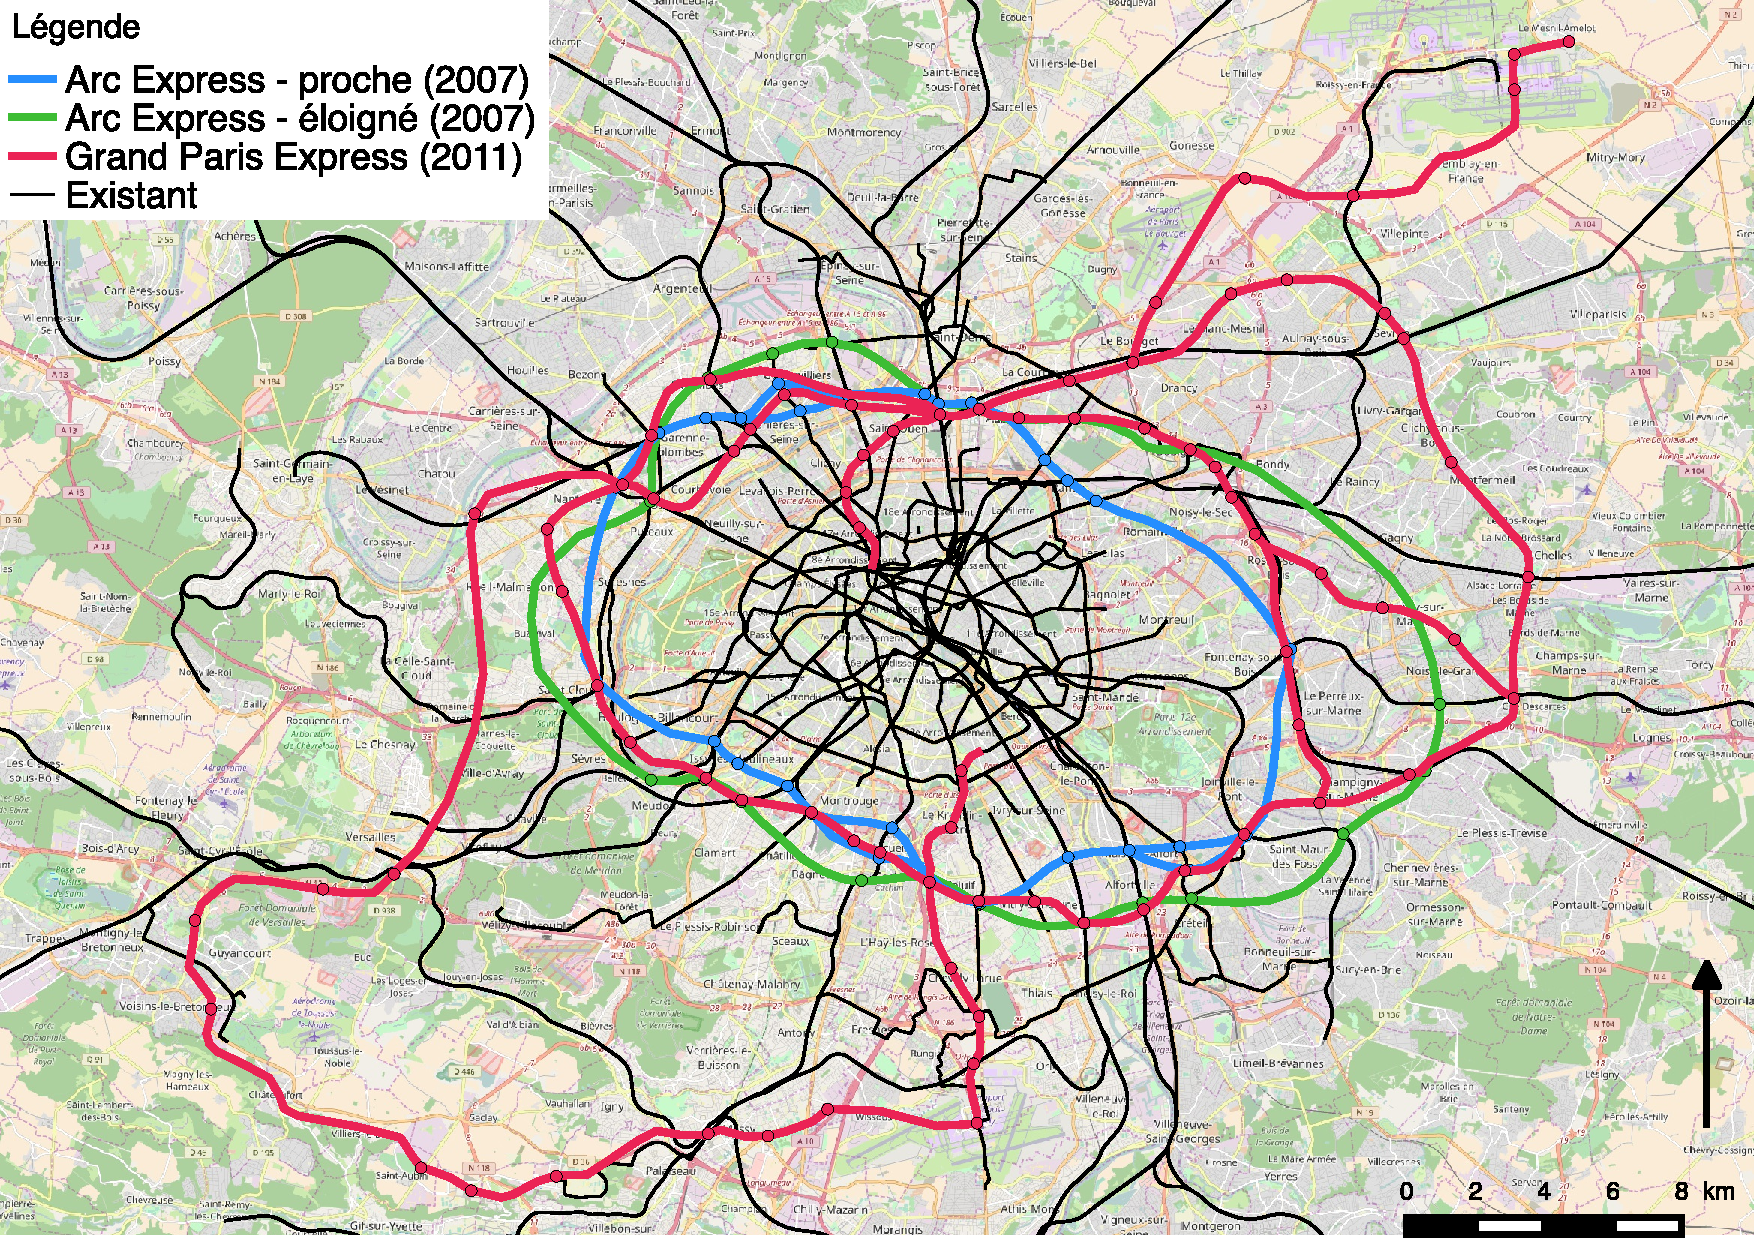
\includegraphics[width=0.8\textwidth]{figures/reseaux}

\medskip

\textit{Projet de transport successifs pour la nouvelle infrastructure de transport du Grand Paris}

}


\sframe{Application: Résultats}{

% We compute for each project accessibility differentials $\Delta T_i$ in average travel time from each IRIS, in comparison with the network without the project. Average travel time accessibility is defined as $T_i = \sum_k \exp{-t_{ik}/t_0}$ with $k$ \emph{Communes}, $t_{ik}$ travek time, and $t_0$ a decay parameter. To each project is associated a date\footnote{2006 for \emph{Arc Express}, 2008 for \emph{Réseau du Grand Paris} and 2010 for \emph{Grand Paris Express}}, corresponding roughly to the mature announcement of the project. It stays a bit arbitrary as it is difficult on the one hand to determine precisely as a planning project does not emerge from nothing in one day, and one the other hand it may correspond to different realities of learning about the project by economic agents (we do therefore the limiting but necessary assumption of a diffusion of information for the majority of agents in a time smaller than a year). We study the lagged correlations of this variable with the variations $\Delta Y_{ij}$ of the following socio-economic variables: population, median income, Gini index for income, average price of real estate transactions and average value of real estate mortgages. A Fisher test is done for each estimation and the value is set to 0 if it is not significant ($p<0.05$ in a classical manner). The study with generalized accessibility in the sense of Hansen has also been conducted but is less interesting as it has a very low sensitivity to the mobility component (network and decay) compared to the variables themselves. It informs therefore only on relations between these and is not presented here. We show in figure~\ref{fig:empiricalres} the results for all networks and variables. It is first remarkable to note the presence of significant effects for all variables. Lower values for the parameter $t_0$ give correlations higher in absolute value, unveiling a possible higher importance of local accessibility on territorial dynamics. The behavior of population shows a clearly detached peak corresponding to 2008, what suggests an impact of the older project \emph{Arc Express} on population growth, the effect of other projects would then be spurious from their proximity in the most important branches. It would imply that areas where they are fundamentally different such as \emph{Plateau de Saclay} are less sensitive to transportation projects, what would confirm the artificial planned aspect of the development of this territory. Concerning income, we observe a similar behavior but in a negative way, what would imply a decrease of wealth linked to the increase of accessibility, however accompanied by a decrease of inequalities. Finally, real estate prices are as expected driven by the potential arrival of new networks. This effect disappear after two years for the \emph{Grand Paris Express}, suggesting a temporal speculation bubble. We demonstrate thus the existence of complex lagged correlation links, that we call causalities in this sense, between territorial dynamics and anticipated dynamics of networks. A finer understanding of working processes is beyond the scope of this paper and would imply for example qualitative fieldwork or targeted case studies. This example shows however the operational potentialities of our method on a real case study.




\centering

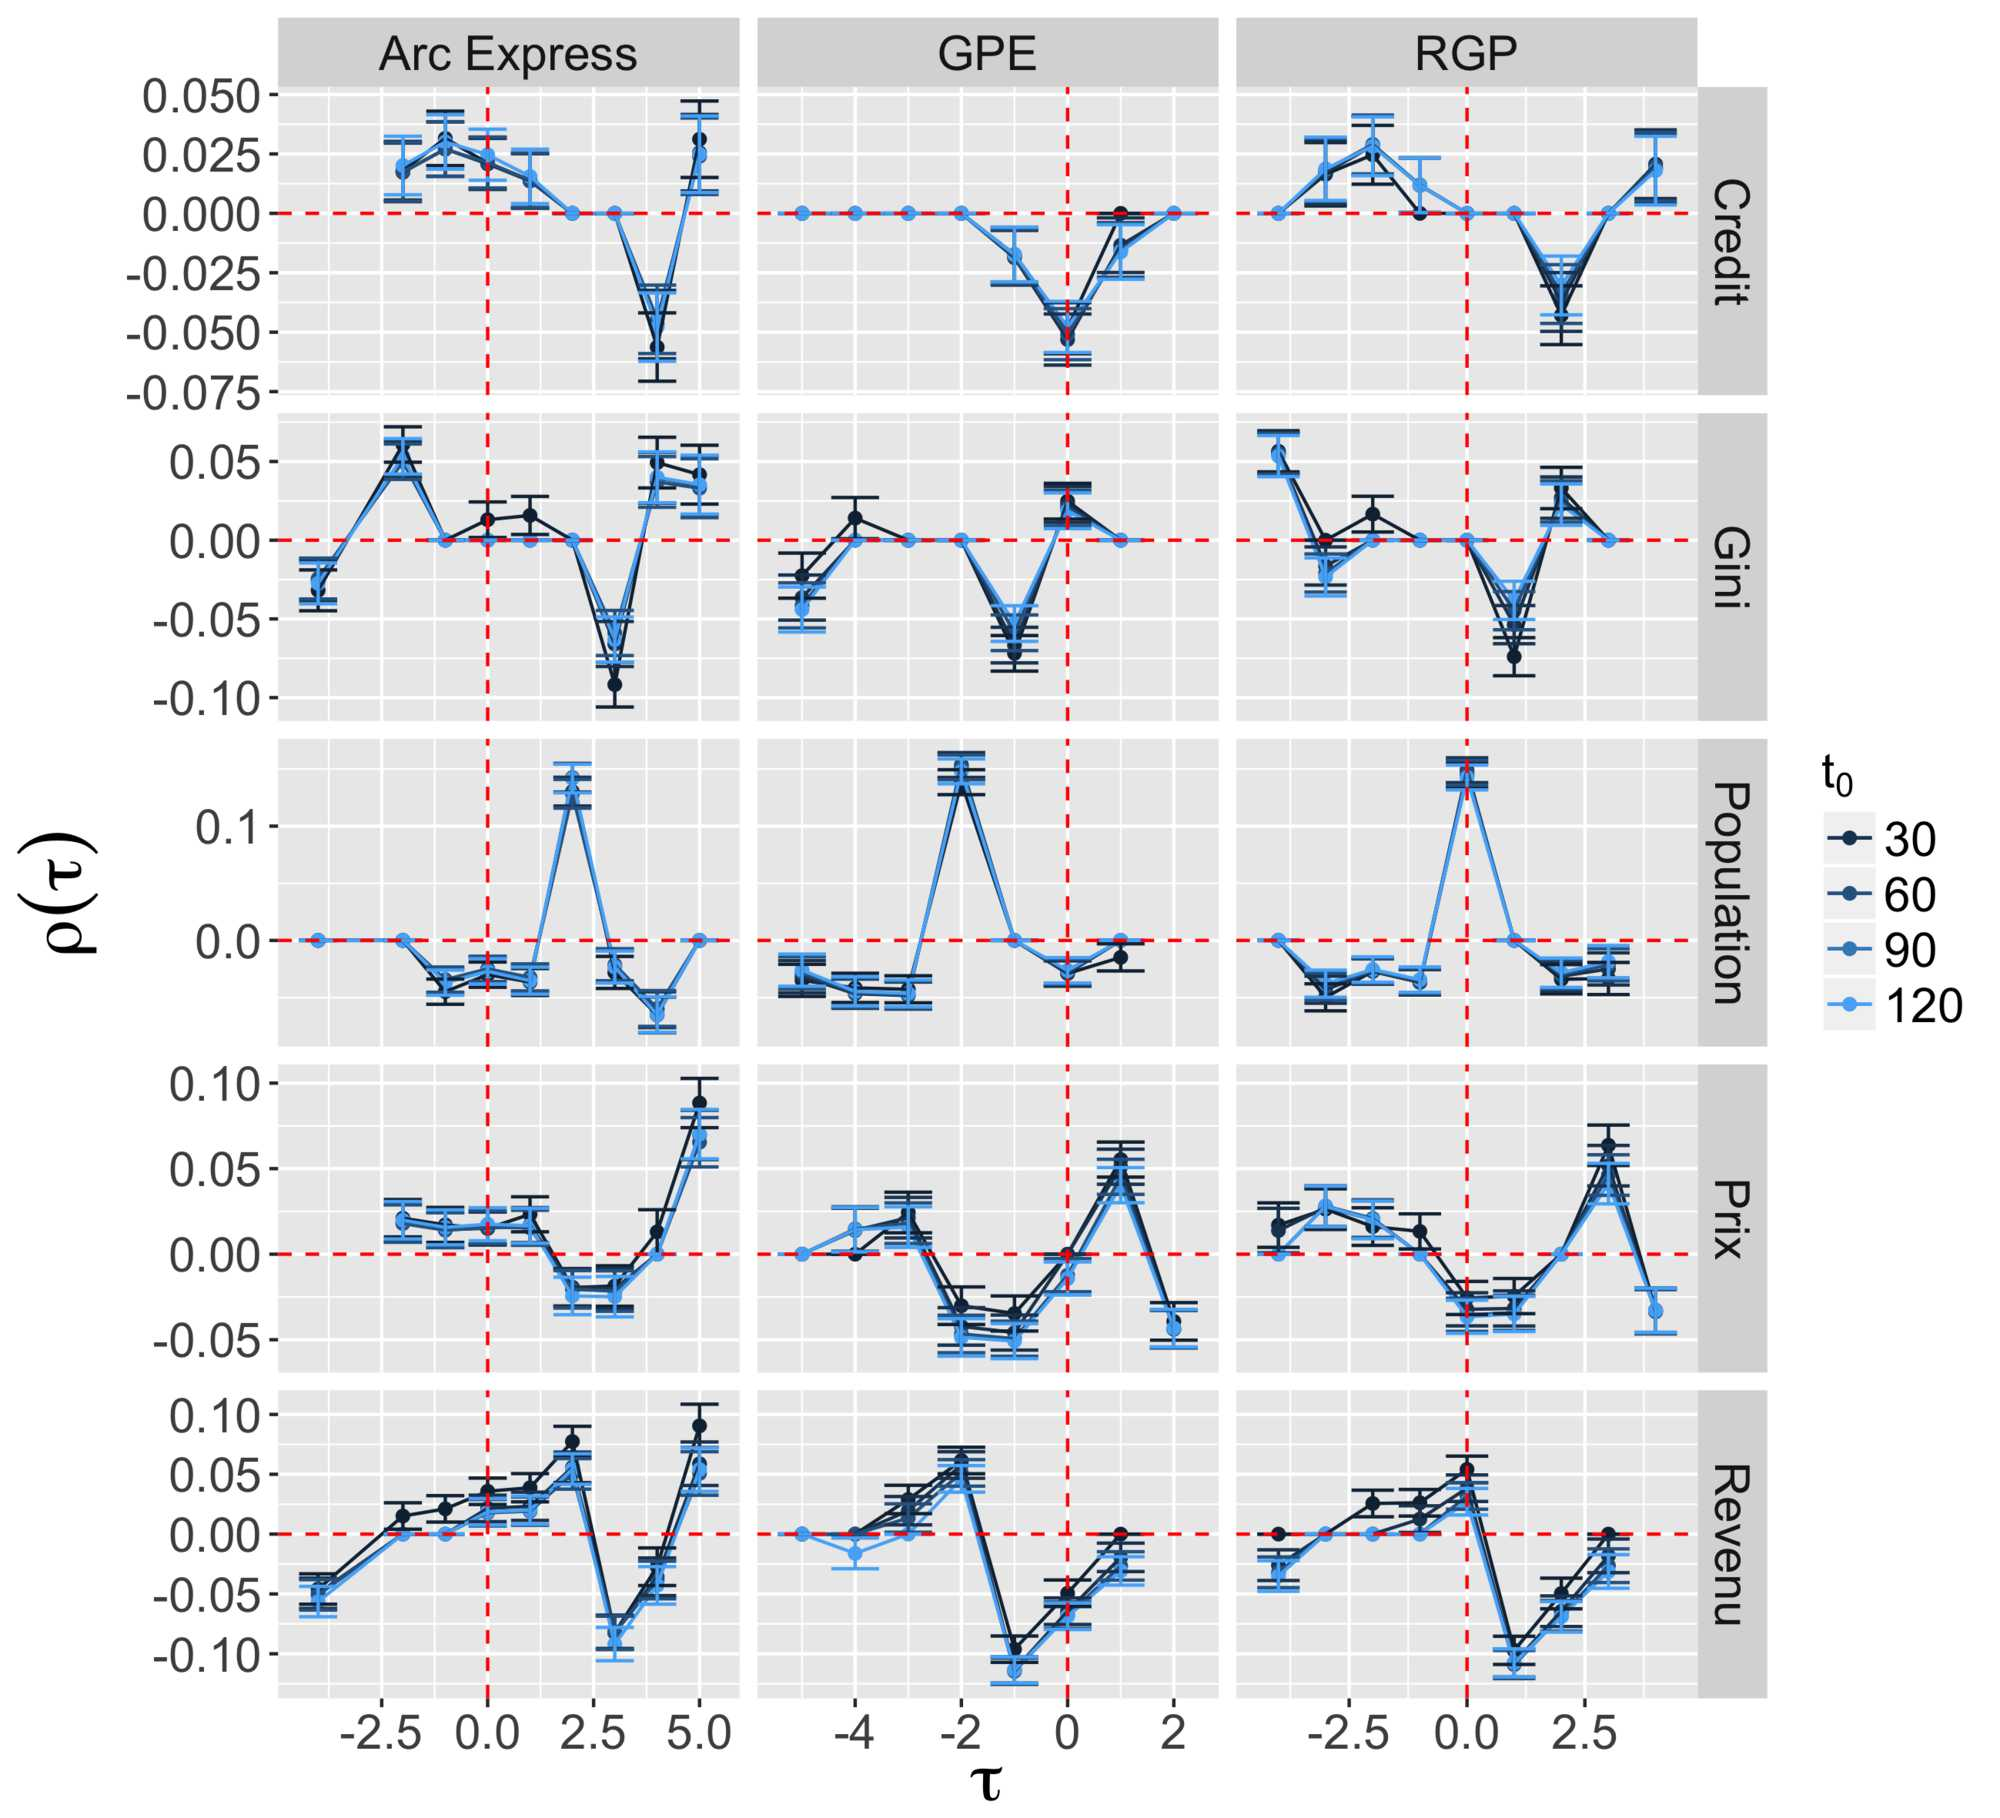
\includegraphics[width=0.62\textwidth]{figures/1-2-1-fig-casestudies-empiricalres}

\textit{Valeurs de $\rho_{\tau}$ pour les différents projets (colonnes) et les différentes variables (lignes), avec les différentiels d'accessibilité}

}



\sframe{Application à l'Afrique du Sud}{

\centering

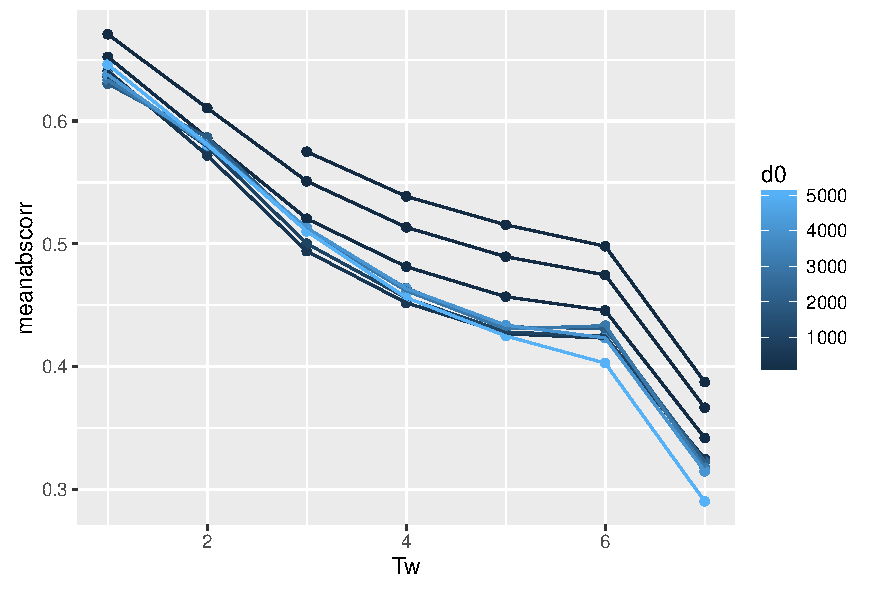
\includegraphics[width=0.5\textwidth]{figures/southafrica_meanabscorrs}
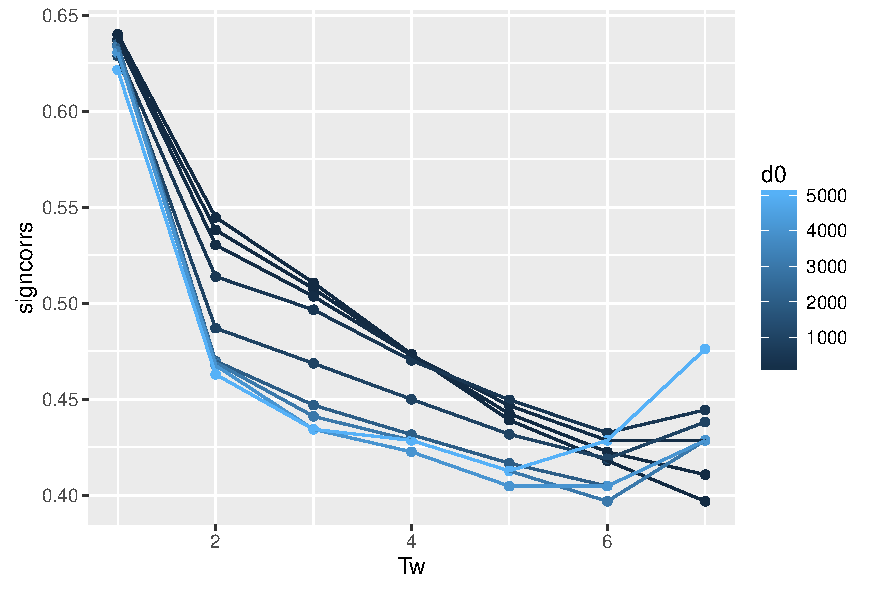
\includegraphics[width=0.5\textwidth]{figures/southafrica_significantcorrs}

\medskip

\textit{Détermination de la fenêtre temporelle et de la portée spatiale de l'accessibilité}


}


\sframe{Application à l'Afrique du Sud}{


\centering

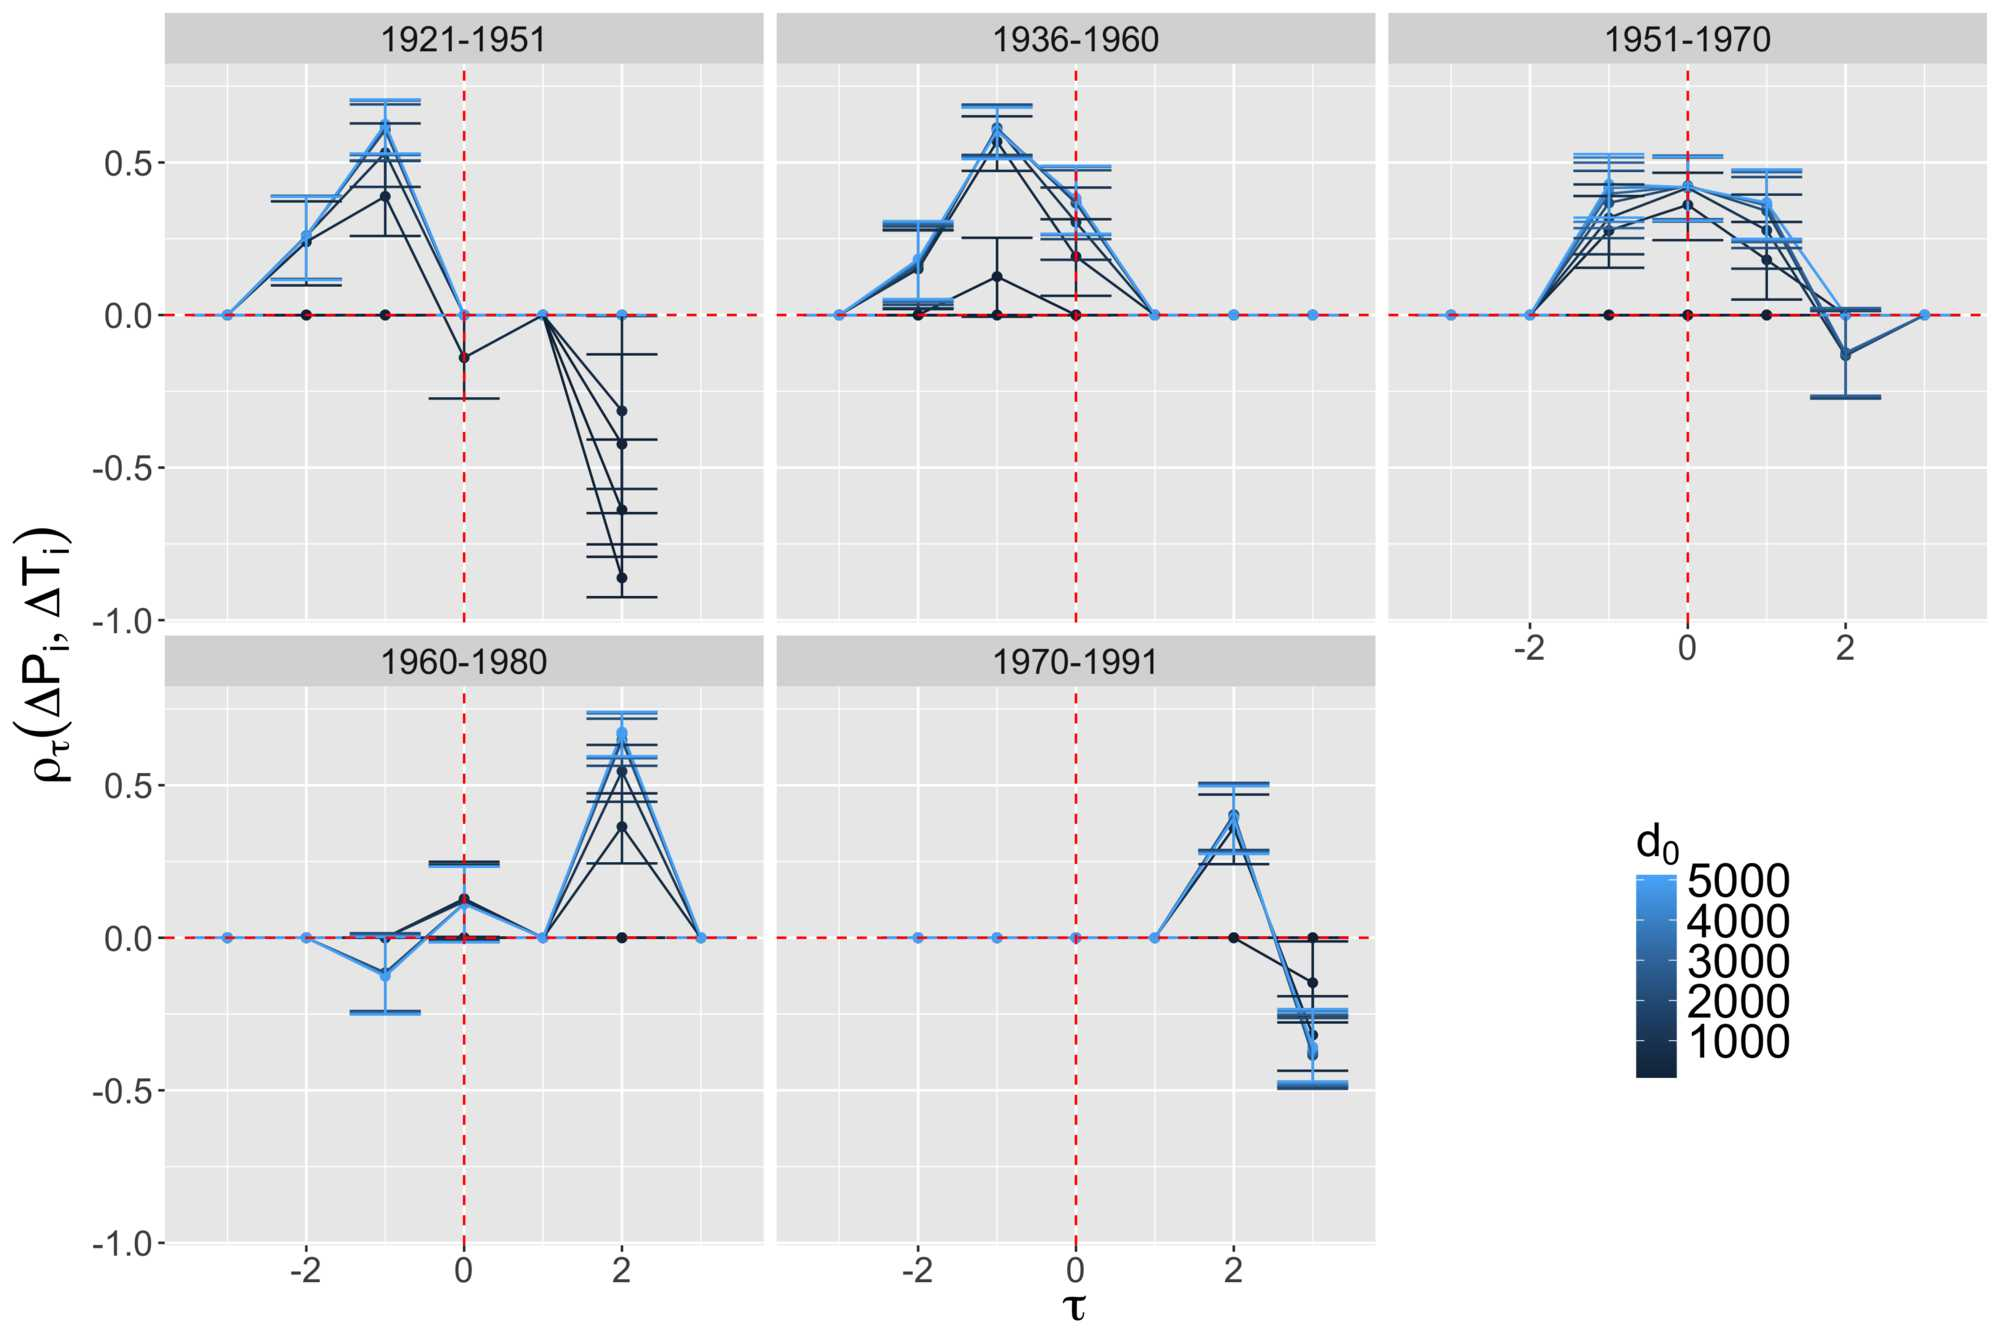
\includegraphics[width=0.82\textwidth]{figures/4-2-3-fig-causalityregimes-sudafcorrs.jpg}

\medskip

\textit{Inversion du sens de la causalité suggère un effet de ségrégation structurelle des politiques d'apartheid}



}


\sframe{Application à la France}{

\centering

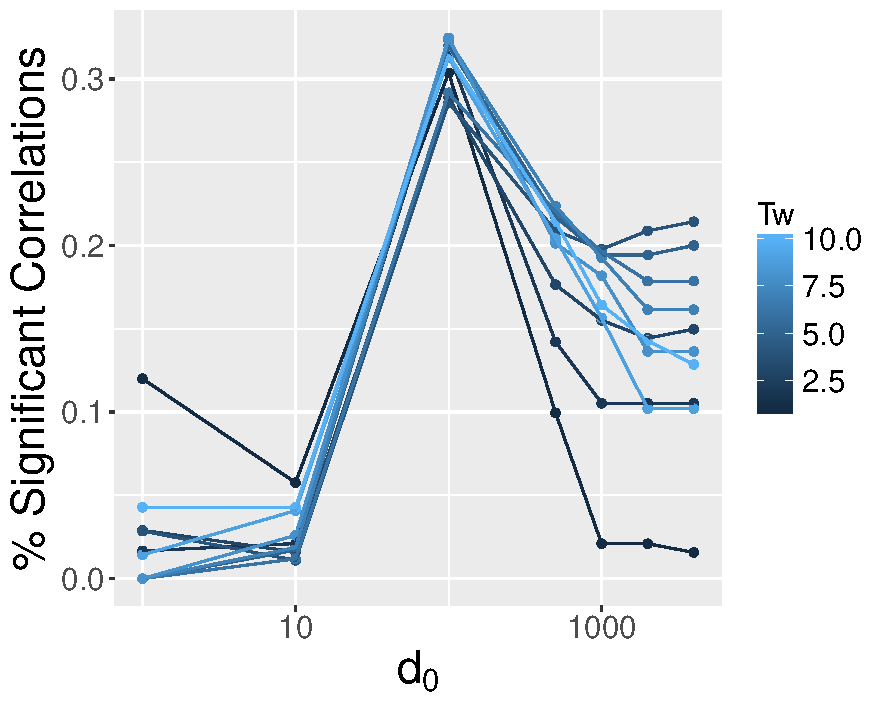
\includegraphics[width=0.5\textwidth]{figures/significantcorrs_d0}
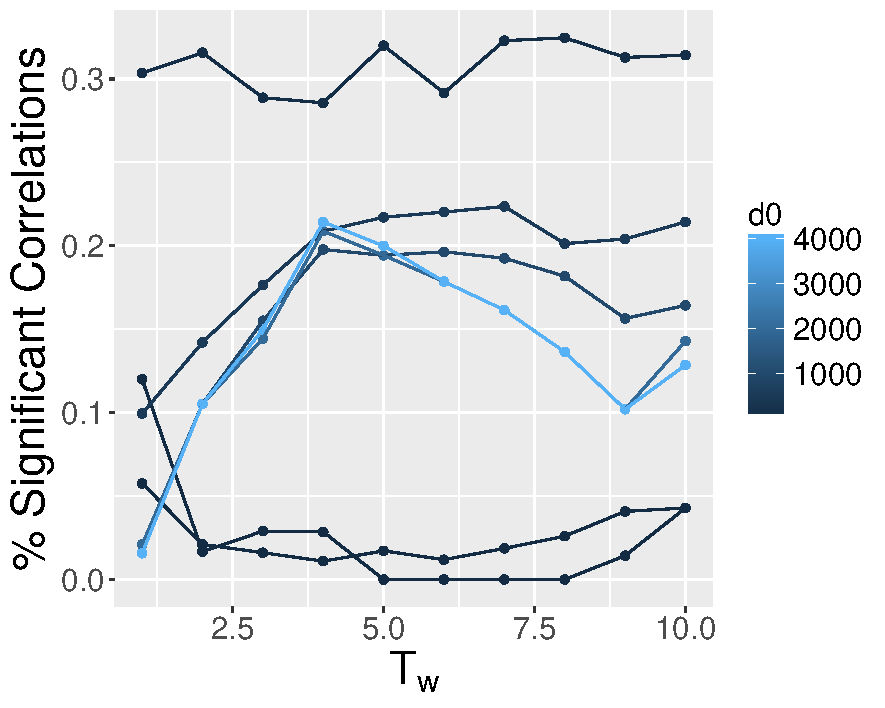
\includegraphics[width=0.5\textwidth]{figures/significantcorrs_Tw}

\medskip

\textit{Fenêtre temporelle et portée spatiale optimales (réseau ferré et population sur la période 1830-1999)}

}

\sframe{Application à la France}{


\centering

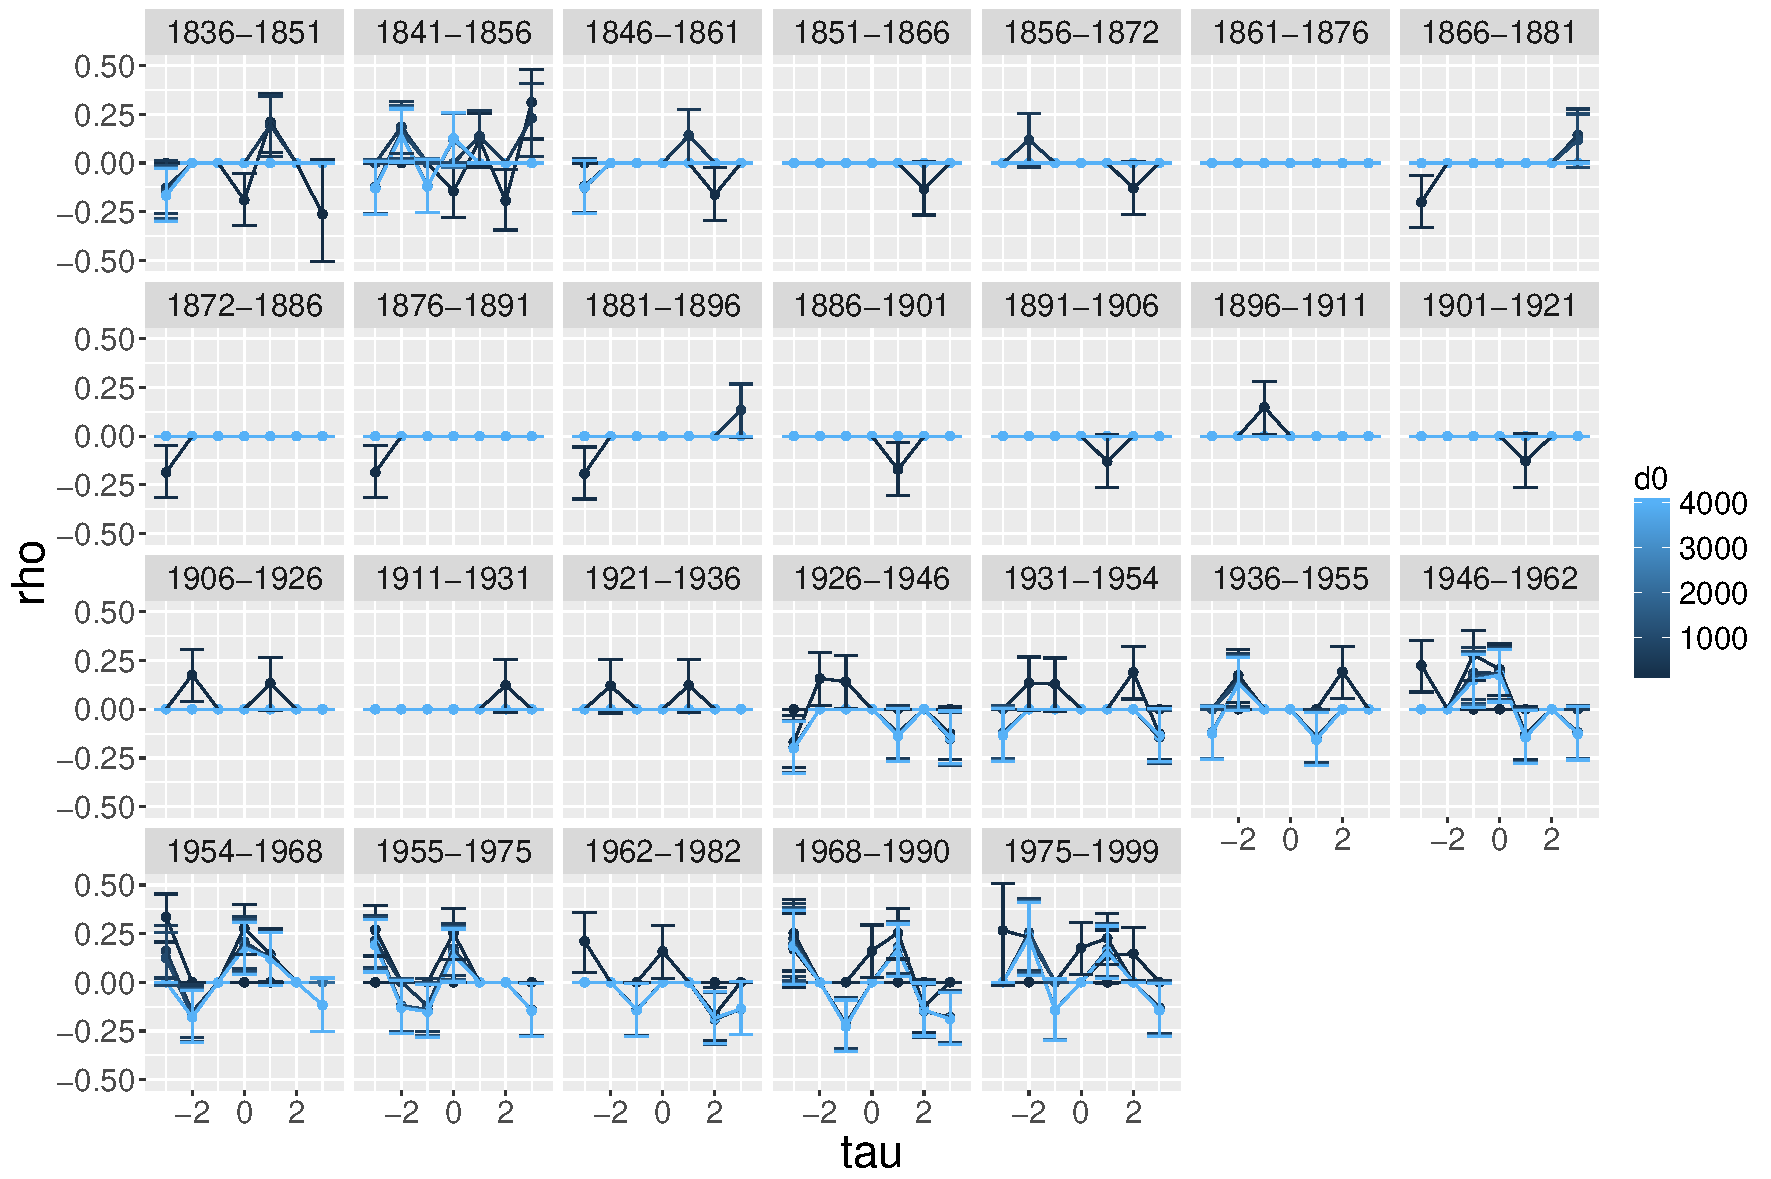
\includegraphics[width=0.82\textwidth]{figures/laggedCorrs_time_Tw4}

\textit{Profils de corrélation : pas de signal significatif}

}







%%%%%%%%%%%%%%%%%
\section{Discussion}
%%%%%%%%%%%%%%%%%


%Nous discutons finalement ces résultats en les plaçant dans la perspective plus large de la co-évolution des réseaux de transport et des territoires, dont nous donnons une définition ainsi que des pistes de modélisation. L'ensemble de ce travail propose ainsi un regard original sur la question des effets structurants des infrastructures de transport.


\sframe{Perspective : co-évolution}{

% def de la coevol

Proposition d'une définition de la co-évolution, basée sur une revue multi-disciplinaire :

\begin{enumerate}
	\item Existence de processus évolutifs : transformations des composantes du système territorial aux différentes échelles
	\item Trois manifestations de la co-évolution à des niveaux emboités :
	\begin{itemize}
		\item Entités en relations causales circulaires
		\item Population d'entités dans une région géographique, identifiable en pratique par les régimes de causalité
		\item Niveau global du système, interdépendance forte
	\end{itemize} 
	\item Existence de sous-systèmes en relative isolation spatio-temporelle où s'opèrent différentes co-évolutions (lien avec le concept de morphogenèse
\end{enumerate}




}


\sframe{Modélisation à l'échelle mesoscopique}{

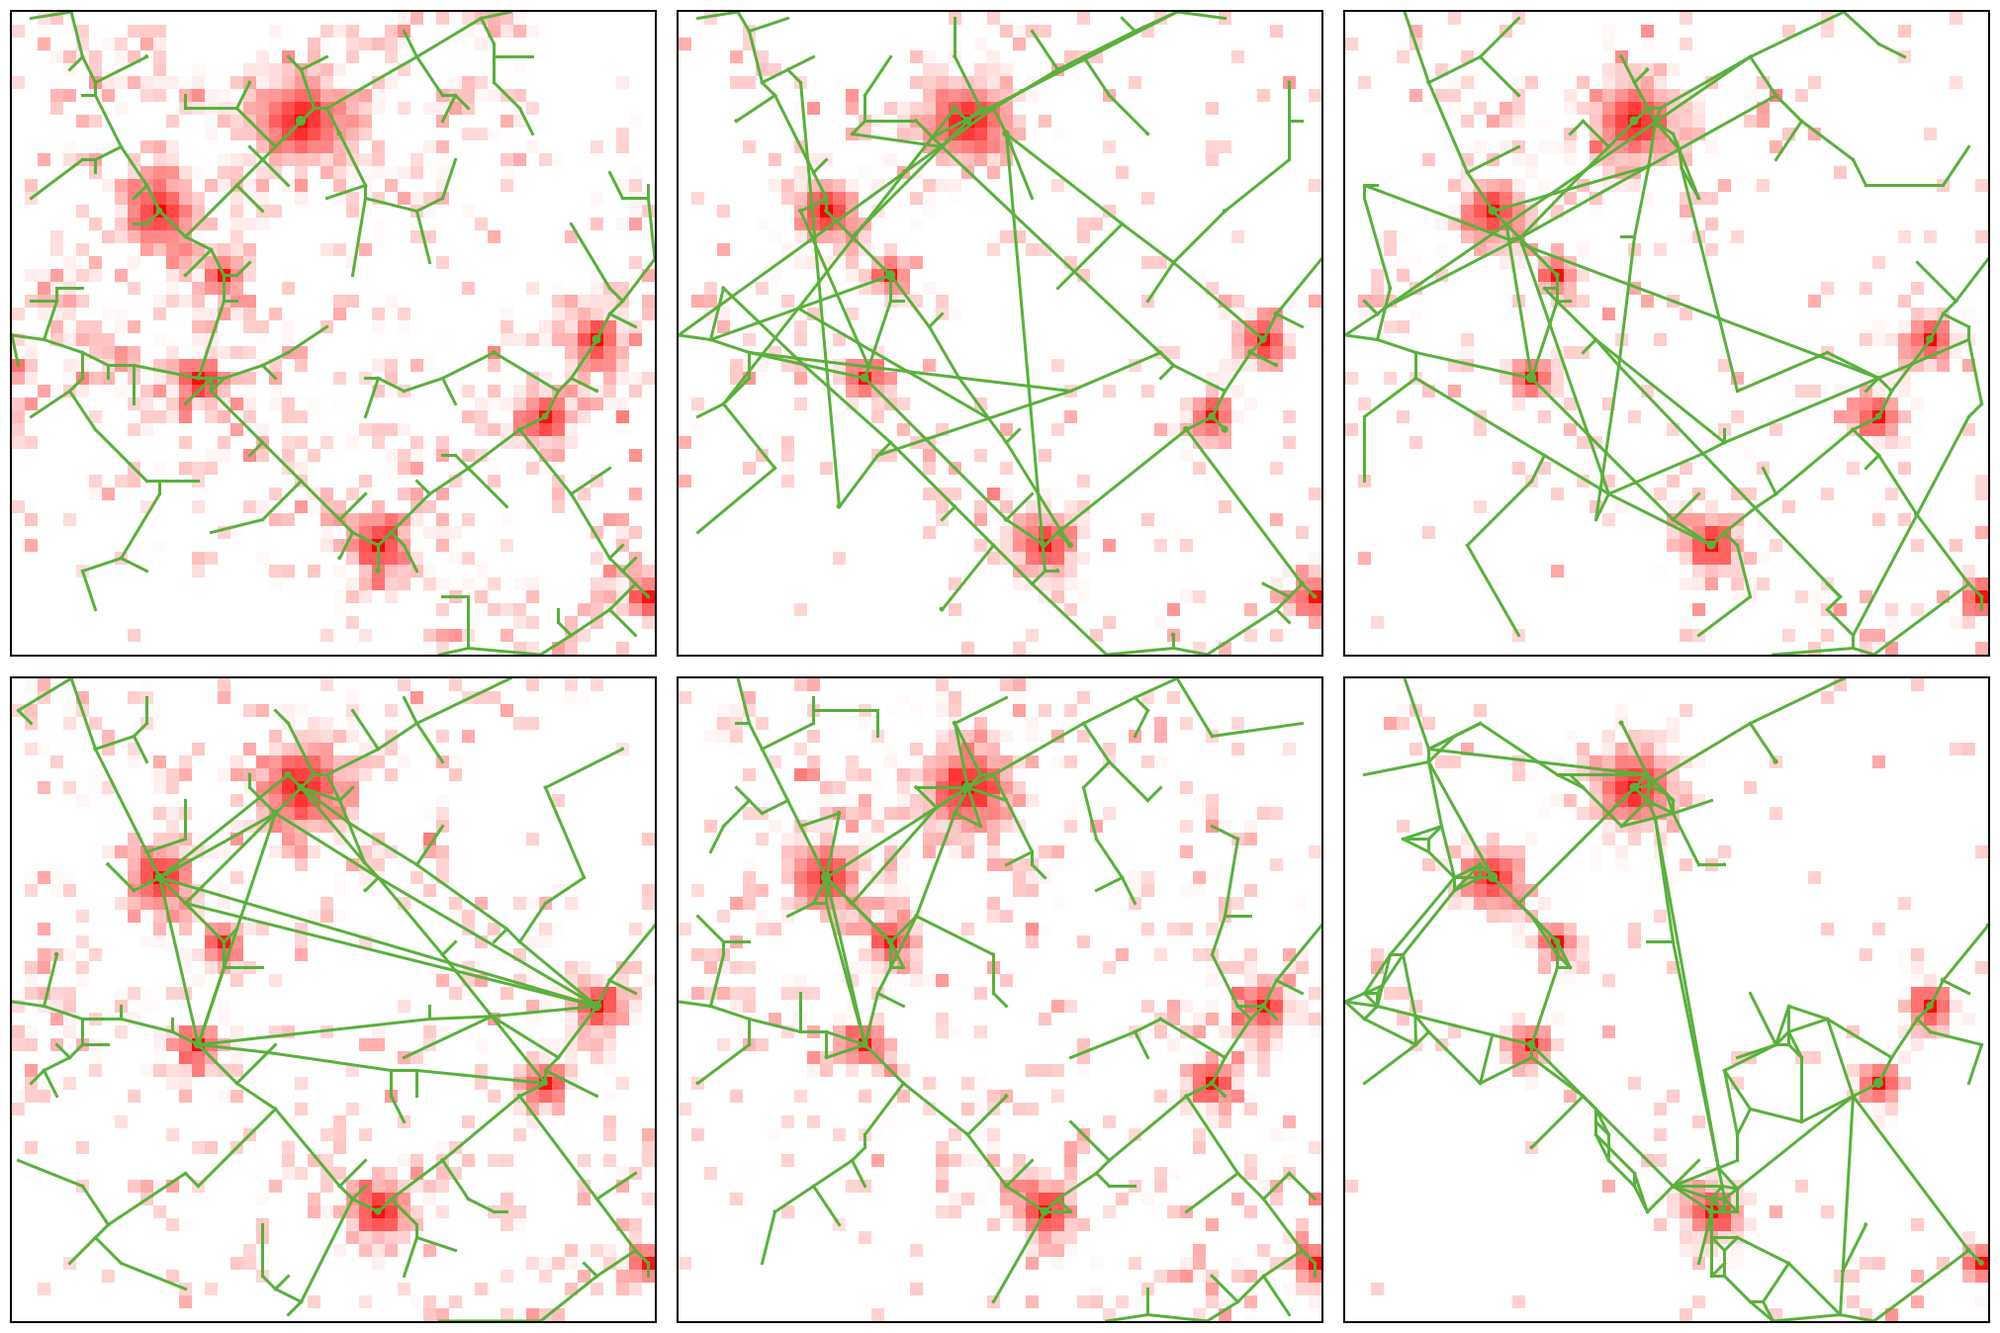
\includegraphics[width=\linewidth]{figures/7-1-2-fig-networkgrowth-examples.jpg}

}



\sframe{Régimes de causalité}{

%\textit{Unsupervised learning on lagged correlations between local variables unveils a diversity of causality regimes in a model co-evolving urban form and network topology}

%$\rightarrow$ Link between \emph{co-evolution regime} and morphogenetic properties of the urban system

\textit{Multi-modélisation pour la croissance du réseau couplée au modèle RBD}

\medskip

\centering

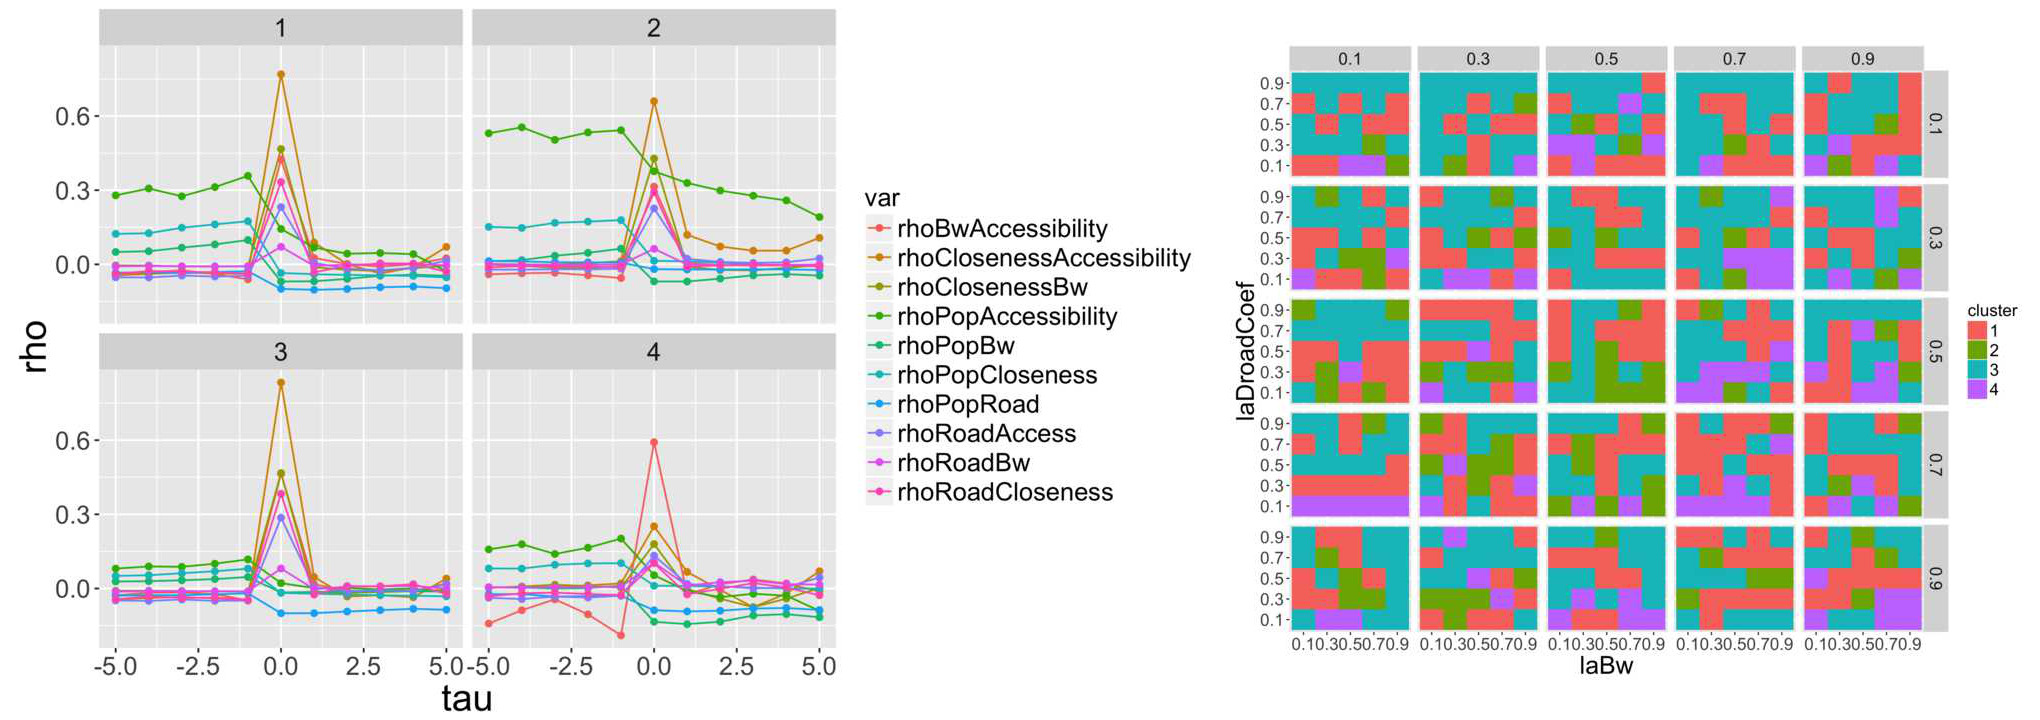
\includegraphics[width=\textwidth]{figures/7-2-2-fig-mesocoevolmodel-causality.jpg}

\footnotesize\textit{(Gauche) Profils de corrélations retardées ; (Droite) Distribution des régimes dans l'espace des paramètres}

}


\sframe{Co-évolution à l'échelle macroscopique}{

\centering

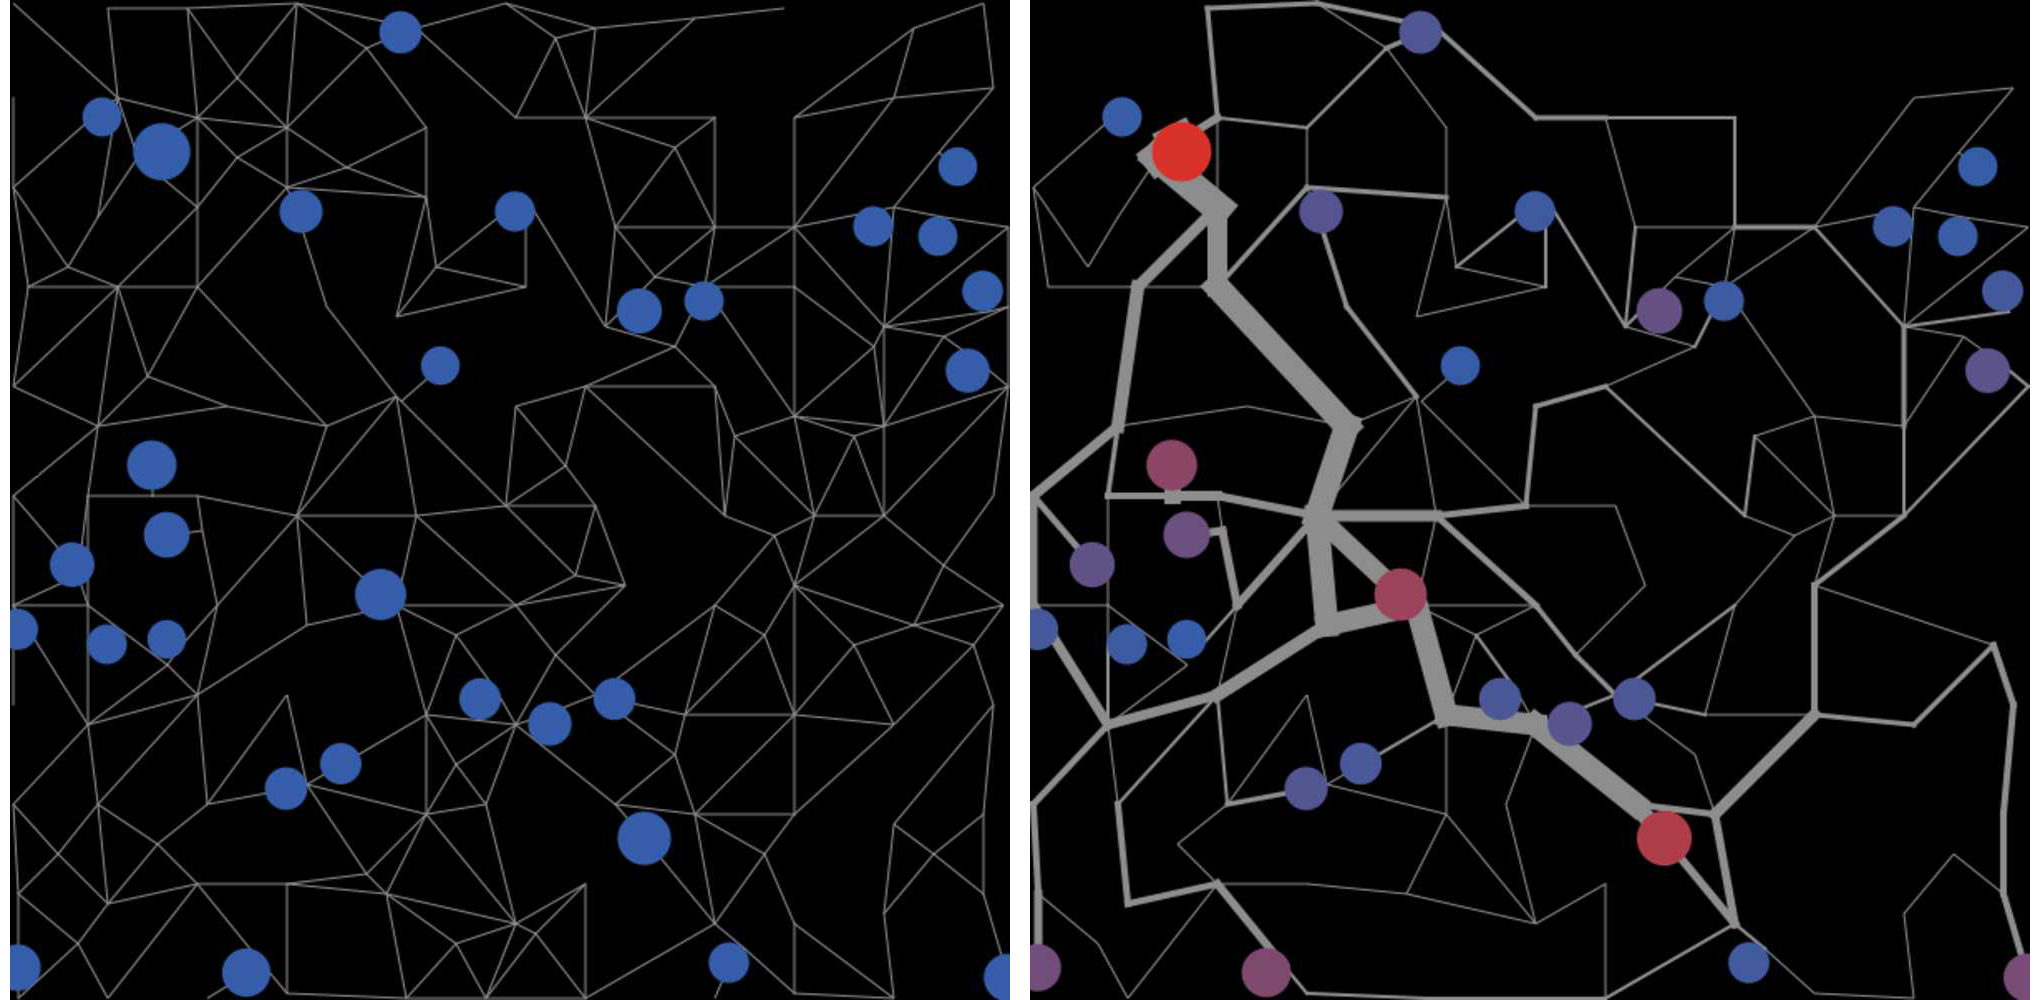
\includegraphics[width=\textwidth]{figures/6-2-3-fig-macrocoevol-slimemould.jpg}

\textit{Modèle d'interaction entre villes~\cite{pumain2017urban} couplé à un modèle d'auto-renforcement de réseau~\cite{tero2010rules}}

}



\sframe{Co-évolution macroscopique : motifs de corrélation}{

\centering

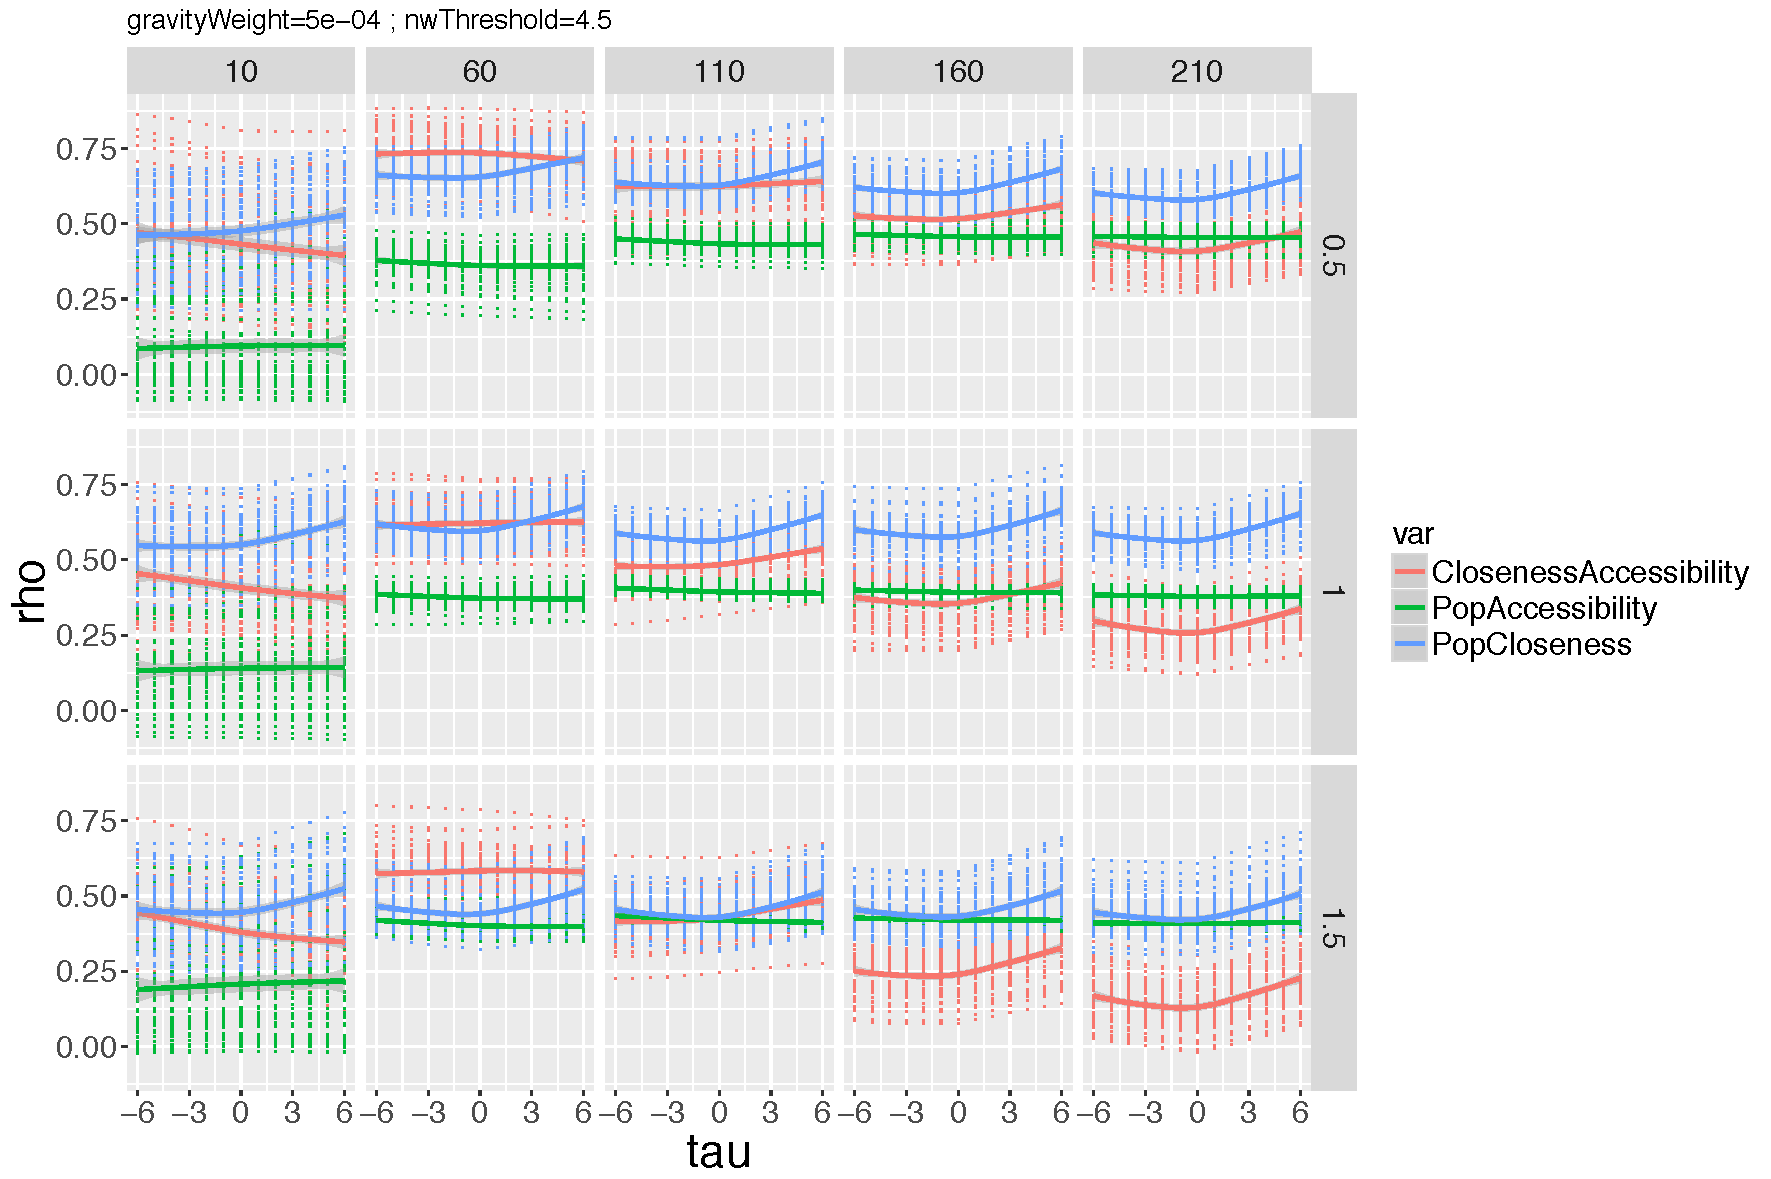
\includegraphics[width=\linewidth]{figures/macrocoevol_laggedcorrs_gravityWeight5e-04_nwThreshold4_5}

}














% The application of our approach must be lead carefully regarding the choice of scales, processes and objects of study. Typically, it will be not adapted to the quantification of spatio-temporal processes for which the temporal scale of diffusion if of the same order than the estimation window, as our stationarity assumption here stays basic. We could propose to proceed to estimations on moving windows but it would then require the elaboration of a spatial correspondence technique to follow the propagation of phenomena. An example of concrete application that would have a strong thematic impact would be a characterization of a fundamental component of the Evolutive Urban Theory that is the hierarchical diffusion of innovation between cities~\cite{pumain2010theorie}. This would be done by analyzing potential spatio-temporal dynamics of patents classifications such as the one introduced by~\cite{10.1371/journal.pone.0176310}. We also underline that these are rather open methodological questions, for which a concretisation is the potential link between the non-ergodic properties of urban systems~\cite{pumain2012urban} and a wave-based characterization of these processes.

%An other direction for developments and potential applications can be found when going to a more local scale, by exploring an hybridation with Geographically Weighted Regression techniques~\cite{brunsdon1998geographically}. The determination by cross-validation of Akaike criterion of an optimal spatial scale for the performance of these models, as done by~\cite{2017arXiv170607467R} in a multi-modeling fashion, could be adapted in our case to determine a local optimal scale on which lagged correlations would be the most significant, what would allow to tackle the question of non-stationarity by a mostly spatial approach.






\sframe{Discussion}{

\justify

\vspace{-1cm}

\textbf{Implications}

$\rightarrow$ Motifs de corrélations retardées pour identifier des ``effets structurants'' dans des systèmes complexes

\medskip

$\rightarrow$ Le concept opérationnel de \textit{Régime de causalité} introduit une nouvelle façon de comprendre la co-évolution dans les modèles de simulation

\bigskip

\textbf{Développements}

$\rightarrow$ Caractérisation de la diffusion spatio-temporelle : test de l'hypothèse de la diffusion spatiale de l'innovation dans la Théorie Evolutive des Villes \cite{pumain2010theorie}

\medskip

$\rightarrow$ Echelles optimales pour la stationnarité : lien avec GWR

\cite{brunsdon1998geographically}

}




\sframe{Conclusion}{


\justify

%We have introduced a generic method of Granger causality on territorial spatio-temporal data, and shown its potentialities and operational nature with synthetic data and on a real case. We postulate that the simple methodological apparel is am asset for a certain level of generality, but that the application to complex case studies exhibiting circular causalities demonstrate the high potential to contribute to the understanding of dynamics for this type of co-evolutive systems.


\justify

$\rightarrow$ Une méthode validée sur données synthétiques et montrée opérationnelle sur des systèmes réels

\medskip

$\rightarrow$ A l'interface des domaines de connaissance : théorie, modélisation, empirique, méthodologique

\medskip

$\rightarrow$ A l'interface des disciplines : analyse spatiale, statistiques, datamining



\bigskip
\bigskip
\bigskip

\footnotesize{ - Code, données et résultats disponibles à\\ \texttt{https://github.com/JusteRaimbault/CityNetwork}\\
- Article sur arXiv à \texttt{https://arxiv.org/abs/1709.08684}\\
- Remerciements : Nous remercions l'\textit{European Grid Infrastructure} et \textit{France-Grilles} en particulier pour le support technique et l'infrastructure.
}

}

% Results obtained in the section 3.1 of this paper have been computed on the virtual organisation \textit{vo.complex-system.eu} of the \textit{European Grid Infrastructure} (\texttt{http://www.egi.eu}). We thank the \textit{European Grid Infrastructure} and its \textit{National Grid Initiatives} (\textit{France-Grilles} in particular) to give the technical support and the infrastructure.





\sframe{Reserve slides}{

\centering

\Large

\textbf{Reserve Slides}

}




\sframe{Granger causality}{

Granger causality test based on VAR processes :

\[
X(t) = \sum_{0 \leq \tau \leq \tau_Y} b_{\tau} Y(t - \tau)
\]

\bigskip

If there exists $b_{\tau}$ such that $\left|b_{\tau}\right|> 0$ significantly, then $Y$ Granger-causes $X$.

\bigskip

We have then $\rho_{\tau}(Y,X) > 0$.


}



\sframe{Morphogenesis}{

\textbf{Morphogenesis} (\textit{Oxford dictionary}) 
\begin{enumerate}
\item \textit{Biology} : The origin and development of morphological characteristics
\item \textit{Geology} : The formation of landforms or other structures.
\end{enumerate}

\bigskip

\textbf{History of the notion}

$\rightarrow$ Started significantly with embryology around 1930~\cite{abercrombie1977concepts} 

$\rightarrow$ Turing's 1952 paper~\cite{turing1952chemical}, linked to the development of Cybernetics

$\rightarrow$ first use in 1871, large peak in usage between 1907-1909, increase until 1990, decrease until today. \textit{Scientific fashion ?}


}


\sframe{Defining Morphogenesis}{

\textbf{Meta-epistemological framework of imbricated notions:}

Self-organization $\supsetneq$ Morphogenesis $\supsetneq$ Autopoiesis $\supsetneq$ Life


\bigskip

\textbf{Properties:}

\begin{itemize}
\item Architecture links form and function
\item Emergence strength~\cite{bedau2002downward} increases with notion depth, as bifurcations~\cite{thom1974stabilite}
\end{itemize}

\bigskip

\textbf{Definition of Morphogenesis :} \textit{Emergence of the form and the function in a strongly coupled manner, producing an emergent architecture \cite{doursat2012morphogenetic}}



}





%%%%%%%%%%%%%%%%%%%%%
\begin{frame}[allowframebreaks]
\frametitle{References}
\bibliographystyle{apalike}
\bibliography{/Users/juste/ComplexSystems/CityNetwork/Biblio/Bibtex/CityNetwork,biblio,biblio_paper}
\end{frame}
%%%%%%%%%%%%%%%%%%%%%%%%%%%%





\end{document}







